\chapter{Multivariable Riemann Integration}
\label{ch:multivariable-integration}

\section{Rectangles, Partitions, and Darboux Sums}

This is the direct extension of Chapter~9: intervals become rectangles,
length becomes volume, and one partitions each coordinate interval at once.
The Darboux definition is unchanged in spirit.  Chapter~10 supplies the
compactness and uniform-continuity facts that make continuous functions
integrable on these higher-dimensional compact rectangles.

We begin with \emph{scalar-valued} functions $f:Q\subseteq\R^n\to\R$.
The tuple $x=(x_1,\ldots,x_n)$ is one point of $Q$, and
$f(x)=f(x_1,\ldots,x_n)$ is one real number. Several variables occur
in the input, not the output. These outputs are ordered real numbers.
For bounded $f$, the set $f(R)\subseteq\R$ is nonempty and bounded on a cell $R$. Completeness
therefore gives its finite infimum and supremum, written
$\inf_{x\in R}f(x)$ and $\sup_{x\in R}f(x)$. Here $x$ is a vector input.
\begin{center}
\begin{tabular}{ll}
Chapter 9 & Chapter 12\\\hline
subinterval & subrectangle\\
length & $n$-dimensional volume\\
$\inf_I f,\ \sup_I f$ & $\inf_R f,\ \sup_R f$
\end{tabular}
\end{center}

\begin{definition}[Rectangles and volume]
A \textbf{rectangle} in $\R^n$ is a product
\[
Q=[a_1,b_1]\times\cdots\times[a_n,b_n],
\]
where
\[
a_j<b_j
\qquad(1\leq j\leq n).
\]
Its \textbf{volume} is
\[
\operatorname{vol}(Q)=\prod_{j=1}^{n}(b_j-a_j).
\]
\end{definition}

\Needspace{15\baselineskip}
\paragraph{A grid you can see.}
On $Q=[0,2]\times[0,1]$, choose horizontal-coordinate cuts
$0=x_0<x_1=1<x_2=2$ and vertical-coordinate cuts
$0=y_0<y_1=1/2<y_2=1$. A typical cell is
$[x_{i-1},x_i]\times[y_{j-1},y_j]$, with area
$(x_i-x_{i-1})(y_j-y_{j-1})$. There are four cells, each of area $1/2$.
\begin{center}
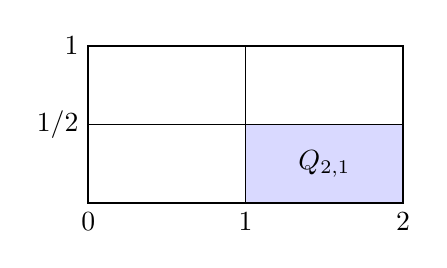
\begin{tikzpicture}[x=2cm,y=2cm]
\fill[blue!15] (1,0) rectangle (2,.5);
\draw[thick] (0,0) rectangle (2,1);
\draw (1,0)--(1,1) (0,.5)--(2,.5);
\node at (1.5,.25) {$Q_{2,1}$};
\node[below] at (0,0) {$0$}; \node[below] at (1,0) {$1$};
\node[below] at (2,0) {$2$};
\node[left] at (0,.5) {$1/2$}; \node[left] at (0,1) {$1$};
\end{tikzpicture}
\end{center}
Higher dimensions add no new idea: partition every coordinate interval and
take products. In general choose
\[
a_j=x_{j,0}<x_{j,1}<\cdots<x_{j,m_j}=b_j\quad(1\leq j\leq n).
\]
The resulting closed cells are
\[
Q_{i_1,\ldots,i_n}=[x_{1,i_1-1},x_{1,i_1}]\times\cdots
\times[x_{n,i_n-1},x_{n,i_n}],\quad 1\leq i_j\leq m_j.
\]
There are $r=\prod_jm_j$ cells. From now on, when only this finite
collection and its volumes matter, suppress the multi-indices and relabel
them $Q_1,\ldots,Q_r$. Then explicitly
\[
Q=\bigcup_{i=1}^r Q_i,\qquad
\operatorname{vol}(Q)=\sum_{i=1}^r\operatorname{vol}(Q_i).
\]
The interiors are pairwise disjoint; shared faces are allowed. The volume
identity follows by expanding the product of the sums of coordinate lengths.
This is the same convention as the closed subintervals in Chapter~9:
shared endpoints caused no problem for Darboux sums, and shared faces cause
none here. We are adding cell volumes, not claiming disjointness of closed sets.
Half-open cells will enter only when an actual step function needs one value
on a shared face.


\begin{definition}[Grid partitions and Darboux sums]
Let $Q$ be a rectangle.  A \textbf{grid partition} of $Q$ is obtained by
choosing a finite partition of each interval $[a_j,b_j]$ and taking all
products of the resulting subintervals.  Its members are \textbf{subrectangles}.
For bounded
\[
f:Q\longrightarrow\R
\]
and a grid partition $\mathcal P=\{Q_1,\ldots,Q_r\}$, put
$m_i=\inf_{Q_i}f$ and $M_i=\sup_{Q_i}f$. Define
\[
U(f,\mathcal P)=\sum_{i=1}^rM_i\operatorname{vol}(Q_i),
\qquad
L(f,\mathcal P)=\sum_{i=1}^rm_i\operatorname{vol}(Q_i).
\]
The function $f$ is \textbf{Riemann integrable} on $Q$ if
\[
\inf_{\mathcal P}U(f,\mathcal P)
=\sup_{\mathcal P}L(f,\mathcal P).
\]
We may subsequently write the same finite sums as $\sum_{R\in\mathcal P}$
when individual cell numbers do not matter. The common value is the multiple Riemann integral (a double integral for
$n=2$, a triple integral for $n=3$), denoted by
\[
\int_Q f(x_1,\ldots,x_n)\,\dd(x_1,\ldots,x_n).
\]
\end{definition}

In scalar-integral notation we abbreviate $x=(x_1,\ldots,x_n)$ and
$\dd x=\dd(x_1,\ldots,x_n)$, writing $\int_Qf(x)\,\dd x$.
This is unsigned scalar Riemann-integration notation. It is distinct from
$\dd x_1\wedge\cdots\wedge\dd x_n$, the oriented top-degree form to be
defined in Chapter~13. The latter is built from the coordinate covectors
of \cref{def:coordinate-differentials}; it retains orientation information
that scalar volume does not.
This is an $n$-variable integral, not integration in the first coordinate.
For $n=2$ we also write $\iint_Qf(x,y)\,\dd A=\int_Qf(x,y)\,\dd(x,y)$;
for $n=3$, $\iiint_Qf(x,y,z)\,\dd V$. These denote scalar coordinate
volume, not identities between differential forms.

\paragraph{Refinement puts approximations on the same grid.}
A refinement adds coordinate cuts and removes none. Every old cell becomes
a finite union of smaller cells. If the coordinate-cut sets of two grids
are $P_j$ and $P'_j$, their common refinement uses $P_j\cup P'_j$ for
every $j$. It therefore refines both grids.
For one coarse cell write the operation out:
\[
R=R_1\cup\cdots\cup R_s,\qquad
\operatorname{vol}(R)=\sum_{k=1}^s\operatorname{vol}(R_k).
\]
Since every $R_k\subseteq R$,
\[
\inf_R f\leq\inf_{R_k}f\leq\sup_{R_k}f\leq\sup_R f.
\]
Multiply by the nonnegative cell volumes and add to get
\[
\begin{split}
(\inf_R f)\operatorname{vol}(R)&\leq
\sum_{k=1}^s(\inf_{R_k}f)\operatorname{vol}(R_k),\\
\sum_{k=1}^s(\sup_{R_k}f)\operatorname{vol}(R_k)&\leq
(\sup_R f)\operatorname{vol}(R).
\end{split}
\]
Summing these inequalities over the coarse cells $Q_1,\ldots,Q_r$ proves
the rule we may now abbreviate:
\[
\mathcal P'\text{ refines }\mathcal P\quad\Longrightarrow\quad
L(f,\mathcal P)\leq L(f,\mathcal P')\leq U(f,\mathcal P')\leq U(f,\mathcal P).
\]
In particular a common refinement shows that every lower sum is at most
every upper sum, even when they originally use different grids.

The definition permits the best lower and upper approximations to come from
different grids. The Darboux criterion says one grid can make them arbitrarily
close: a common refinement puts two separately good approximations onto one grid.
This follows the proof of \cref{prop:darboux-criterion}. The new geometric
step is taking the union of the cut sets in \emph{each} coordinate direction;
the supremum--infimum argument that follows is unchanged.



\begin{proposition}[Darboux criterion]
\label{prop:multivariable-darboux}
A bounded function $f:Q\to\R$ is Riemann integrable if and only if, for every $\eps>0$, there is a grid partition $\mathcal P$ such that
\[
U(f,\mathcal P)-L(f,\mathcal P)<\eps.
\]
\end{proposition}
\begin{proof}
Refining a grid partition decreases upper sums and increases lower sums.
Thus every lower sum is at most every upper sum.  If the two extremal values
are equal, choose partitions whose upper and lower sums are within
\[
\eps/2
\]
of that common value and take their common refinement.  Conversely, the
displayed condition forces the difference of the two extremal values to be
smaller than every positive $\eps$, hence zero by
\cref{lem:positive-small}.
\end{proof}

Choose one tag $\xi_i\in Q_i$ per cell. The familiar tagged sum is
\[
S(f,\mathcal P,\xi)=\sum_{i=1}^r f(\xi_i)\operatorname{vol}(Q_i).
\]
Each sampled height lies between its cell infimum and supremum, so
$L(f,\mathcal P)\leq S(f,\mathcal P,\xi)\leq U(f,\mathcal P)$.
Lower sums approximate from below and upper sums from above. Refinement
narrows their uncertainty; when both reach the same number, the integral
is determined.
\begin{example}[A four-cell calculation]
For $f(x,y)=x+y$ on $[0,1]^2$, split each axis at $1/2$.
\[
\begin{array}{c|c|c|c}
\text{cell (lower left corner)}&\text{area}&\inf f&\sup f\\\hline
(0,0)&1/4&0&1\\
(1/2,0)&1/4&1/2&3/2\\
(0,1/2)&1/4&1/2&3/2\\
(1/2,1/2)&1/4&1&2
\end{array}
\]
Hence
\[
L=\frac{0+\frac12+\frac12+1}{4}=\frac12,
\qquad
U=\frac{1+\frac32+\frac32+2}{4}=\frac32.
\]
On an $m$-by-$m$ equal grid the heights on cell $(i,j)$ are
$(i+j)/m$ and $(i+j+2)/m$, $0\leq i,j<m$. Finite summation gives
$L=1-1/m$, $U=1+1/m$. Refinement narrows the gap to $2/m$ and squeezes
the integral to $1$, using the definition without Fubini.
\end{example}
\begin{center}
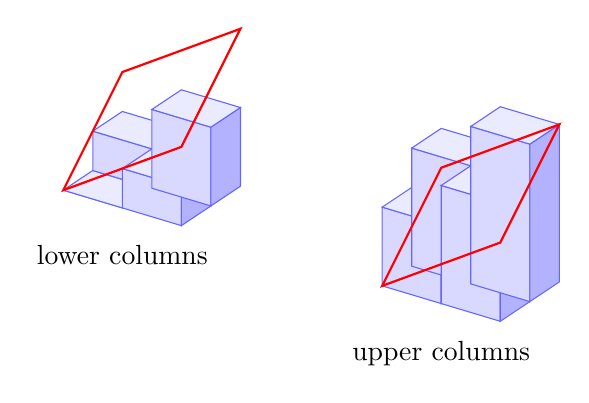
\begin{tikzpicture}[x={(1.5cm,-.45cm)},y={(.75cm,.5cm)},z={(0cm,1cm)}]
\foreach \offset/\upper/\title in {0/0/lower,2.7/1/upper}{
\begin{scope}[shift={(\offset,0,0)}]
\foreach \i in {0,1}{\foreach \j in {0,1}{
\pgfmathsetmacro{\ht}{(\i+\j)/2+\upper}
\filldraw[fill=blue!15,draw=blue!60] ({\i/2},{\j/2},0)--({(\i+1)/2},{\j/2},0)--({(\i+1)/2},{\j/2},\ht)--({\i/2},{\j/2},\ht)--cycle;
\filldraw[fill=blue!30,draw=blue!60] ({(\i+1)/2},{\j/2},0)--({(\i+1)/2},{(\j+1)/2},0)--({(\i+1)/2},{(\j+1)/2},\ht)--({(\i+1)/2},{\j/2},\ht)--cycle;
\filldraw[fill=blue!8,draw=blue!60] ({\i/2},{\j/2},\ht)--({(\i+1)/2},{\j/2},\ht)--({(\i+1)/2},{(\j+1)/2},\ht)--({\i/2},{(\j+1)/2},\ht)--cycle;
}}
\draw[red,thick] (0,0,0)--(1,0,1)--(1,1,2)--(0,1,1)--cycle;
\node[below] at (.5,0,-.35) {\title\ columns};
\end{scope}}
\end{tikzpicture}
\end{center}
The red outline is $z=x+y$ on $[0,1]^2$. On each of the four cells,
the lower column stops at the minimum and the upper column at the maximum.
Each base has area $1/4$; the total column volumes are $1/2$ and $3/2$.


Define the mesh $|\mathcal P|=\max_{R\in\mathcal P}\operatorname{diam}(R)$.
Subtracting the finite sums displays their gap:
\[
\boxed{U(f,\mathcal P)-L(f,\mathcal P)
=\sum_{R\in\mathcal P}\operatorname{osc}_R(f)\operatorname{vol}(R).}
\]
Here $\operatorname{osc}_R(f)=\sup_R f-\inf_R f$. Small oscillations on
all cells make the total gap small.
For later estimates distinguish the cell oscillation
$\operatorname{osc}_R(f)=\sup_R f-\inf_R f$ from the pointwise
oscillation $\omega_f(a)$ of Chapter~9. For a continuous function on a
compact domain $K$, its modulus of continuity is instead
\[
\mu_f(\delta)=\sup\{|f(x)-f(y)|:x,y\in K,\ \|x-y\|\leq\delta\}.
\]
Uniform continuity gives $\mu_f(\delta)\to0$ as $\delta\to0$, and
$\operatorname{osc}_R(f)\leq\mu_f(\operatorname{diam}R)$ for $R\subseteq K$.
The inputs to these three notions are respectively a cell, a point, and a
nonnegative scalar distance.

The proof of \cref{thm:continuous-riemann-integrable} now has a precise
translation: interval length becomes $\operatorname{vol}(Q)$, and interval
mesh becomes maximum cell diameter. Uniform continuity still supplies one
oscillation bound for all cells; summing their volumes gives the global gap.
\begin{theorem}[Continuous functions are integrable]
\label{thm:continuous-multivariable-riemann}
Every continuous function
\[
f:Q\longrightarrow\R
\]
is Riemann integrable.
\end{theorem}
\begin{proof}
Small cells give small oscillation on every cell, hence
a small total Darboux gap. Compactness makes $f$ bounded and uniformly
continuous, so $\mu_f(\delta)\to0$. For every cell,
\[
\operatorname{osc}_R(f)\leq\mu_f(\operatorname{diam}R)\leq\mu_f(|\mathcal P|).
\]
The gap identity and finite volume additivity give
\[
U(f,\mathcal P)-L(f,\mathcal P)\leq
\mu_f(|\mathcal P|)\operatorname{vol}(Q).
\]
Equal subdivisions in each coordinate make the mesh arbitrarily small.
The right side tends to zero, so the Darboux criterion applies.
\end{proof}

\begin{example}[Continuity succeeds; boundedness alone fails]
On $Q=[0,1]^2$, the function $f(x,y)=x^2+y^2$ is integrable by
\cref{thm:continuous-multivariable-riemann}.  In contrast, define
\[
g(x,y)=\begin{cases}1,&x\in\Q,\\0,&x\notin\Q.\end{cases}
\]
Every nondegenerate subrectangle contains points of both kinds, so its
oscillation is $1$.  Consequently every grid partition satisfies
\[
U(g,\mathcal P)-L(g,\mathcal P)=\operatorname{vol}(Q)=1,
\]
and $g$ is not Riemann integrable.  The example separates boundedness from
integrability in several variables just as the Dirichlet function does in
one variable.
\end{example}

\paragraph{Actual bounding functions: owned cells.}
The basic Darboux construction is now in place. Later proofs need actual
bounding functions, not only numerical sums. If two neighboring cells
carry different constants, a shared face would receive conflicting values.
Only for this purpose do we assign every face to one cell.
Partition each coordinate interval at finitely many points. For bookkeeping,
assign each partition point to the interval on its right, except the final
endpoint, which belongs to the last interval. Products of these half-open
intervals (with their final endpoints included) give genuinely disjoint
\emph{owned cells} covering $Q$. Their volumes are the products of their
side lengths, the same as those of their closures.
A rectangular step function $s:Q\to\R$ takes a constant value $c_R$
on each owned cell. Define its step integral by
\[
\int_Qs=\sum_R c_R\operatorname{vol}(R).
\]
This is height times length in one dimension, height times area in two,
and height times $n$-dimensional volume in general. Refining a cell gives
$c\operatorname{vol}(R)=\sum_j c\operatorname{vol}(R_j)$, so refinement
does not change the answer. Two representations have a common refinement;
on each owned refined cell their values agree. Thus this definition is
independent of representation, without any theory of null sets.

For bounded $f$, use on each owned cell the infimum and supremum over
its \emph{closed} rectangle to define $s^-_{\mathcal P}$ and
$s^+_{\mathcal P}$. Then $s^-_{\mathcal P}\leq f\leq s^+_{\mathcal P}$,
and their step integrals are exactly the lower and upper sums defined above.
Closed rectangles in Darboux sums retain their shared faces; the ownership
rule is used to make the step functions single-valued.


\begin{proposition}[Compatibility with preliminary step integration]
\label{prop:step-compatibility}
Every owned-cell rectangular step function is Darboux integrable, with
integral equal to its preliminary step sum.
\end{proposition}
\begin{proof}
The ownership convention changes values only on finitely
many jump planes. Thin strips around those planes make their possible
Darboux contribution arbitrarily small.
Let $I_s$ be the preliminary sum and $M$ a bound for $|s|$. Given any
grid $\mathcal P$, refine it together with the step grid using the union
of their coordinate cuts. Each refined owned cell belongs to one owned
cell of each grid. Its constant value lies between the infimum and
supremum on the closed $\mathcal P$-cell containing it. Multiply by its
volume and add. Common owned-cell refinement preserves $I_s$, so
\[
L(s,\mathcal P)\leq I_s\leq U(s,\mathcal P).
\]
Now include the finitely many jump planes and nearby parallel planes in
a grid. The closed cells touching jump planes lie in thin grid strips of
total volume $\delta$, as small as desired: each strip volume is its
width times a fixed product of side lengths. Elsewhere $s$ is constant
on each closed cell. Therefore $U-L\leq2M\delta$. The Darboux criterion
proves integrability. The preceding squeeze for these grids identifies
its integral with $I_s$. If $M=0$ the conclusion is immediate.
\end{proof}


\begin{theorem}[Basic properties]
\label{thm:multivariable-integral-properties}
If $f,g:Q\to\R$ are integrable and $c\in\R$, then
\[
\int_Q(f+g)\,\dd x
=\int_Qf\,\dd x+\int_Qg\,\dd x,
\qquad
\int_Qcf\,\dd x
=c\int_Qf\,\dd x.
\]
If
\[
f\leq g,
\]
then their integrals have the same order.  Also,
\[
\left\lvert\int_Qf\,\dd x\right\rvert
\leq
\int_Q\abs f\,\dd x,
\]
and
\[
\left\lvert\int_Qf\,\dd x\right\rvert
\leq M\operatorname{vol}(Q)
\]
whenever
\[
\abs{f(x)}\leq M
\qquad(x\in Q).
\]
\end{theorem}
\begin{proof}
\textbf{Strategy.} Place both candidate sums of integrals between common
Darboux bounds, then shrink the gap.

The upper and lower sum inequalities used in the proof of
\cref{thm:integral-properties} hold verbatim for subrectangles:
\[
U(f+g,\mathcal P)\leq U(f,\mathcal P)+U(g,\mathcal P),
\]
\[
L(f+g,\mathcal P)\geq L(f,\mathcal P)+L(g,\mathcal P).
\]
Taking a common refinement of partitions that make the two individual gaps
small proves integrability of the sum. Both $\int_Q(f+g)$ and
$\int_Qf+\int_Qg$ lie in
\[
[L(f,\mathcal P)+L(g,\mathcal P),\ U(f,\mathcal P)+U(g,\mathcal P)].
\]
The length is the sum of the two individual Darboux gaps and can be made
arbitrarily small on one common refinement. This proves equality.
Scalar multiplication and order preservation are identical to
the one-variable arguments.

For absolute values and the two bounds, follow the proof of
\cref{thm:integral-additivity-absolute}, with volume in place of length.
The inequality
\[
\bigl\lvert\abs u-\abs v\bigr\rvert\leq\abs{u-v}
\]
shows from a common partition that $\abs f$ is integrable.  Since
\[
-\abs f\leq f\leq\abs f,
\]
order preservation gives the first estimate.  The second follows by
integrating the constant functions $-M$ and $M$.
\end{proof}




\subsection{Rectangular restriction, gluing, and translation}
The basic multiple Riemann integral has now been constructed. The next
lemmas are bookkeeping tools for cutting a rectangle into finitely many
pieces, enlarging its container, or translating it. Later they support
Jordan regions and change of variables. The gluing argument generalizes
the interval additivity in \cref{thm:integral-additivity-absolute}:
inserting a division point becomes inserting subdivision planes.
\begin{lemma}[Grid restriction and finite gluing]\label{lem:grid-gluing}
Let $Q_1,\ldots,Q_N$ be the closed subrectangles of a finite grid in $Q$.
A bounded $f:Q\to\R$ is integrable exactly when each restriction is,
and then
\[
\int_Q f=\sum_{i=1}^N\int_{Q_i}f.
\]
\end{lemma}
\begin{proof}
Write $Q=Q_1\cup\cdots\cup Q_N$, with disjoint interiors and possible
shared faces. Insert all subdivision planes into any testing grid. Each refined cell
belongs to one $Q_i$, although their closed faces can be shared. Upper
and lower sums are exactly the sums of the corresponding local sums:
explicitly, for the induced local grids $\mathcal P_i$,
\[
L(f,\mathcal P)=\sum_{i=1}^N L(f|_{Q_i},\mathcal P_i),\qquad
U(f,\mathcal P)=\sum_{i=1}^N U(f|_{Q_i},\mathcal P_i).
\]
Every small cell contributes its height times its volume to exactly one
local sum; shared closed faces do not add any extra cell volume.
If $f$ is integrable, make its total nonnegative gap small; each local
gap is at most that total, proving restriction. Conversely choose a grid
on each $Q_i$ with gap below $\eps/N$ and extend all its coordinate cuts
through $Q$. Refinement decreases local gaps, so the total is below $\eps$.
The criterion gives gluing. The sum of the local integrals and the global
integral both lie between the same total lower and upper sums with
arbitrarily small gap, proving additivity of the integral, not merely volume.
\end{proof}

\begin{lemma}[Face strips and zero extension]\label{lem:rectangle-zero-extension}
A bounded function supported on finitely many coordinate hyperplane
sections of a rectangle is integrable with integral zero. If $Q\subseteq P$
are rectangles and $f$ is integrable on $Q$, its extension by zero to $P$
is integrable and has the same integral.
\end{lemma}
\begin{proof}
For the first assertion, put every supporting plane and neighboring
parallel cuts into a grid. All cells with a nonzero value lie in strips
of total volume $\delta\to0$. With bound $M$, the lower and upper sums
are between $-M\delta$ and $M\delta$, and their gap is at most $2M\delta$.
The criterion and squeeze prove the assertion directly from grids.
For extension, subdivide $P$ at the faces of $Q$. On the central rectangle
the restriction is $f$. On every other subrectangle it is zero except
possibly on shared faces of $Q$. The first assertion gives integral zero
there, even though the function need not vanish on the closed shared face.
Grid gluing and additivity now prove the claim. For two unrelated
containing rectangles, enlarge both to a common rectangle.
\end{proof}

\begin{lemma}[Translation of rectangular integrals]\label{lem:integral-translation}
For $a\in\R^n$, set $Q+a=\{x+a:x\in Q\}$ and $g(y)=f(y-a)$ there.
Then $g$ is integrable exactly when $f$ is, and $\int_{Q+a}g=\int_Qf$.
\end{lemma}
\begin{proof}
Translate every coordinate cut by the corresponding coordinate of $a$.
This gives a bijection of grids preserving side lengths and cell volumes.
The value set of $g$ on $R+a$ equals that of $f$ on $R$, so the lower
and upper sums agree exactly. Taking their extrema proves the assertion.
\end{proof}

\begin{definition}[Vector-valued Riemann integrals]
For $f=(f_1,\ldots,f_m):Q\to\R^m$, say $f$ is integrable when every
scalar component is integrable, and define
\[
\int_Qf=\left(\int_Qf_1,\ldots,\int_Qf_m\right)\in\R^m.
\]
There is no natural total order on $\R^m$ corresponding to the scalar
order used by Darboux sums; this is a componentwise extension of the
already constructed scalar integral.
\end{definition}
\begin{proposition}[Linearity of vector integration]
For integrable $f,g:Q\to\R^m$, scalars $a,b$, and a linear map
$T:\R^m\to\R^k$, the functions $af+bg$ and $T\circ f$ are integrable and
\[
\int_Q(af+bg)=a\int_Qf+b\int_Qg,\qquad
\int_QT(f(x))\,\dd x=T\left(\int_Qf(x)\,\dd x\right).
\]
Continuous vector-valued functions on $Q$ are integrable.
\end{proposition}
\begin{proof}
Apply scalar linearity to each component. If $[T]=(t_{ij})$, the $i$th
component of $T\circ f$ is $\sum_jt_{ij}f_j$, whose integral is
$\sum_jt_{ij}\int_Qf_j$. Continuity also passes to each component, so
\cref{thm:continuous-multivariable-riemann} proves the last assertion.
\end{proof}

\section{Iterated Integration}

The equality of an integral over a rectangle with repeated one-variable
integrals is not a new definition.  It is a theorem saying that the same
finite rectangular approximations can be grouped in either order.  The
continuity hypothesis keeps the oscillation on every sufficiently small
product rectangle under control.

\begin{center}
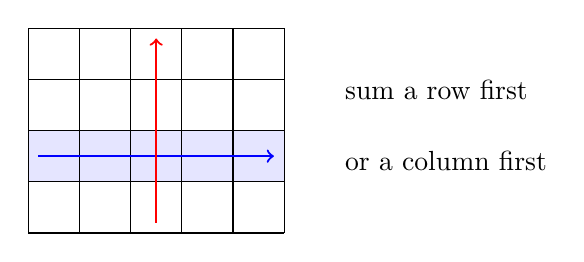
\begin{tikzpicture}[scale=.65]
\fill[blue!10] (0,1) rectangle (5,2);
\draw[step=1] (0,0) grid (5,4);
\draw[->,blue,thick] (.2,1.5)--(4.8,1.5);
\draw[->,red,thick] (2.5,.2)--(2.5,3.8);
\node[anchor=west] at (6,2.8) {sum a row first};
\node[anchor=west] at (6,1.4) {or a column first};
\end{tikzpicture}
\end{center}
A finite rectangular grid has the same total whether its terms are added
row by row or column by column. Riemann--Fubini passes this finite
regrouping to a limit; the estimates ensure both limiting operations
describe the same integral.
A \emph{multiple integral} is the directly defined Riemann integral over
a multidimensional rectangle. An \emph{iterated integral} performs successive
integrations. On $Q=[a,b]\times[c,d]$, $\iint_Qf\,\dd A$ is defined
by two-dimensional grids, whereas $\int_a^b(\int_c^df(x,y)\,\dd y)\,\dd x$
is a later computational representation. Fubini proves their equality
under its hypotheses; it does not define the multiple integral.

For $A\subseteq\R^p$, $B\subseteq\R^q$, write
$x=(x_1,\ldots,x_p)$ and $y=(y_1,\ldots,y_q)$. With $x$ fixed,
$f(x,\cdot):B\to\R$ is a scalar function of $q$ variables.
Its integral $g(x)=\int_B f(x,y)\,\dd y$ is one real number, defining
$g:A\to\R$. The integral $\int_A g(x)\,\dd x$ handles the remaining
$p$ variables. In order, these operations are
\[
f(x,y)\ \xrightarrow{\text{integrate in }y\text{ with }x\text{ fixed}}\
g(x)\ \xrightarrow{\text{integrate in }x}\ \text{a scalar}.
\]
For general $p,q$, either stage can itself be a multiple integral.


\begin{center}
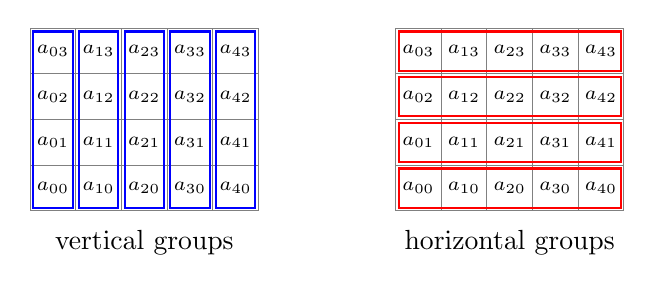
\begin{tikzpicture}[scale=.58]
\foreach \off/\kind in {0/0,8/1}{
\begin{scope}[shift={(\off,0)}]
\draw[step=1,gray] (0,0) grid (5,4);
\foreach \i in {0,...,4}{\foreach \j in {0,...,3}{
\node[font=\scriptsize] at (\i+.5,\j+.5) {$a_{\i\j}$};}}
\ifnum\kind=0
\foreach \i in {0,...,4}{\draw[blue,thick] (\i+.07,.07) rectangle (\i+.93,3.93);}
\node[below] at (2.5,-.2) {vertical groups};
\else
\foreach \j in {0,...,3}{\draw[red,thick] (.07,\j+.07) rectangle (4.93,\j+.93);}
\node[below] at (2.5,-.2) {horizontal groups};
\fi
\end{scope}}
\end{tikzpicture}
\end{center}
Both pictures contain exactly the same twenty contributions:
$\sum_i\sum_j a_{ij}=\sum_j\sum_i a_{ij}$. With $a_{ij}$ equal to a
tagged function value times cell volume, this is the finite model behind
Riemann--Fubini. The theorem justifies passing from that identity to integrals.

\begin{theorem}[Riemann--Fubini theorem for continuous functions]
\label{thm:riemann-fubini}
Let
\[
Q=A\times B,
\]
where $A\subseteq\R^p$ and $B\subseteq\R^q$ are rectangles, and let
\[
f:Q\longrightarrow\R
\]
be continuous.  Then the functions
\[
x\longmapsto\int_Bf(x,y)\,\dd y,
\qquad
y\longmapsto\int_Af(x,y)\,\dd x
\]
are continuous, and
\[
\int_{A\times B}f(x,y)\,\dd(x,y)
=
\int_A\left(\int_Bf(x,y)\,\dd y\right)\dd x
=
\int_B\left(\int_Af(x,y)\,\dd x\right)\dd y.
\]
\end{theorem}
\begin{proof}
Every section is continuous on its rectangle, so its integral exists.
Write $a=\operatorname{vol}(A)>0$, $b=\operatorname{vol}(B)>0$, and
$G(x)=\int_B f(x,y)\,\dd y$. The bounded-integral estimate gives
\[
|G(x')-G(x)|\leq b\sup_{y\in B}|f(x',y)-f(x,y)|.
\]
Uniform continuity of $f$ makes the supremum less than $\eps/b$ whenever
$x'$ is sufficiently close to $x$, proving continuity of $G$.
Thus its outer integral also exists.

\textbf{Strategy.} The section integral and the multiple integral lie
between the same product Darboux sums. For a product cell $R\times S$ put
$m_{R,S}=\inf_{R\times S}f$ and $M_{R,S}=\sup_{R\times S}f$.
For $x\in R$, integration over the $S$ cells gives
\[
\sum_Sm_{R,S}\operatorname{vol}(S)\leq G(x)
\leq\sum_SM_{R,S}\operatorname{vol}(S).
\]
Integrate over $R$ and add, using rectangular restriction and gluing:
\[
L(f,\mathcal P_A\times\mathcal P_B)\leq\int_A G
\leq U(f,\mathcal P_A\times\mathcal P_B).
\]
The multiple integral lies in this same interval. Uniform continuity of
$f$ gives arbitrarily small product Darboux gaps, so the two integrals
agree. Reverse the coordinate blocks to prove continuity of the other
section-integral function and its integral identity.
\end{proof}



\begin{example}[A double integral on a rectangle]
For the continuous function $f(x,y)=x+2y$ on $[0,1]\times[0,2]$,
Riemann--Fubini gives
\begin{align*}
\int_{[0,1]\times[0,2]}(x+2y)\,\dd(x,y)
&=\int_0^1\left(\int_0^2(x+2y)\,\dd y\right)\dd x\\
&=\int_0^1(2x+4)\,\dd x=5.
\end{align*}
Here the rectangle makes iterated integration natural; no coordinate change
is needed.
\end{example}

\subsection{Beyond continuous integrands}
Continuity is sufficient, but not necessary, for the equality of multiple
and iterated integrals. It buys us two conveniences: every section is
integrable, and its integral varies continuously with the parameter.
For a bounded $f:A\times B\to\R$ that is merely Riemann integrable,
a section $f(x,\cdot):B\to\R$ need not be integrable for every $x$.
Thus $x\mapsto\int_B f(x,y)\,\dd y$ may not even be defined everywhere.
The multiple integral still makes sense; the difficulty lies in requiring
an ordinary Riemann integral on every slice.

\begin{definition}[Lower and upper section integrals]
\label{def:section-darboux-integrals}
Let $A\subseteq\R^p$ and $B\subseteq\R^q$ be compact rectangles and
$f:A\times B\to\R$ bounded. Define functions on $A$ by
\[
\underline I_B(x)=\underline{\int_B}f(x,y)\,\dd y
 :=\sup_{\mathcal P_B}L(f(x,\cdot),\mathcal P_B),\qquad
\overline I_B(x)=\overline{\int_B}f(x,y)\,\dd y
 :=\inf_{\mathcal P_B}U(f(x,\cdot),\mathcal P_B).
\]
Define functions on $B$ by reversing the roles:
\[
\underline I_A(y)=\sup_{\mathcal P_A}L(f(\cdot,y),\mathcal P_A),\qquad
\overline I_A(y)=\inf_{\mathcal P_A}U(f(\cdot,y),\mathcal P_A).
\]
All partitions here are grid partitions of the indicated rectangle.
These are Darboux integrals, whether or not the sections are integrable.
\end{definition}
If $|f|\leq K$, both functions on $A$ lie between
$-K\operatorname{vol}(B)$ and $K\operatorname{vol}(B)$.
Common refinement gives $\underline I_B\leq\overline I_B$; equality
at $x$ holds exactly when $f(x,\cdot)$ is Riemann integrable.
The same statements hold with $A,B$ interchanged.

\begin{theorem}[Darboux--Fubini theorem for a Riemann-integrable function]
\label{thm:darboux-fubini}
Let $f:A\times B\to\R$ be Riemann integrable on a product of compact
rectangles. All four lower and upper section-integral functions are
Riemann integrable on their parameter rectangles, and
\[
\begin{aligned}
\int_A\underline I_B(x)\,\dd x
 &=\int_A\overline I_B(x)\,\dd x=\int_{A\times B}f,\\
\int_B\underline I_A(y)\,\dd y
 &=\int_B\overline I_A(y)\,\dd y=\int_{A\times B}f.
\end{aligned}
\]
No hypothesis of section integrability is imposed.
\end{theorem}
\begin{proof}
Take grid partitions $\mathcal P_A,\mathcal P_B$. For their product cells put
\[
m_{R,S}=\inf_{R\times S}f,\qquad M_{R,S}=\sup_{R\times S}f.
\]
For each $x\in R$, comparison with the section sums gives
\[
\sum_Sm_{R,S}\operatorname{vol}(S)
\leq\underline I_B(x)\leq\overline I_B(x)
\leq\sum_SM_{R,S}\operatorname{vol}(S).
\]
Indeed the left sum is at most the section's lower sum on $\mathcal P_B$,
which is at most its lower integral; the upper comparison is the reverse.
For either $h=\underline I_B$ or $h=\overline I_B$, take the infimum and
supremum over $x\in R$, multiply by $\operatorname{vol}(R)$, and sum:
\[
L(f,\mathcal P_A\times\mathcal P_B)
\leq L(h,\mathcal P_A)\leq U(h,\mathcal P_A)
\leq U(f,\mathcal P_A\times\mathcal P_B).
\]
The cross bounds also give
\[
L(f,\mathcal P_A\times\mathcal P_B)
\leq L(\underline I_B,\mathcal P_A)
\leq U(\overline I_B,\mathcal P_A)
\leq U(f,\mathcal P_A\times\mathcal P_B).
\]
Every grid partition of $A\times B$ is such a product: separate its first
$p$ coordinate-cut lists from its last $q$ lists. Integrability of $f$
therefore supplies product grids with gap smaller than any prescribed
$\eps>0$. The first chain bounds the outer Darboux gap for each $h$ by
this gap, proving its integrability by \cref{prop:multivariable-darboux}.
Both $\int_Ah$ and $\int_{A\times B}f$ lie between the same product
lower and upper sums. Their difference has absolute value less than
$\eps$, so they agree. For the other order, hold $y\in S$ fixed and use
\[
\sum_Rm_{R,S}\operatorname{vol}(R)
\leq\underline I_A(y)\leq\overline I_A(y)
\leq\sum_RM_{R,S}\operatorname{vol}(R).
\]
Taking extrema on $S$ and summing with weights $\operatorname{vol}(S)$
proves integrability and the same equality on $B$.
Only finite Darboux sums and the Darboux criterion have been used.
\end{proof}

\begin{corollary}[Ordinary iterated integrals]
\label{cor:ordinary-iterated-riemann}
Under the hypotheses of \cref{thm:darboux-fubini}, if every section
$f(x,\cdot)$ is Riemann integrable, then
$G(x)=\int_Bf(x,y)\,\dd y$ is Riemann integrable on $A$ and
\[
\int_{A\times B}f=\int_A G(x)\,\dd x.
\]
The corresponding conclusion holds in the reverse order. If every section
in both directions is integrable, both iterated integrals exist and equal
the multiple integral.
\end{corollary}
\begin{proof}
Section integrability says $G=\underline I_B=\overline I_B$.
Apply the theorem, and interchange the coordinate blocks for the other order.
\end{proof}
The continuous theorem remains the main computational case: continuity
automatically supplies every section integral, and even continuity of $G$.

\begin{example}[A dense family of nonintegrable sections]
\label{ex:thomae-dirichlet-sections}
Recall Thomae's function from \cref{ex:thomae-function}, writing it as
$t$ on $[0,1]$: $t(x)=0$ at irrational
$x$ and $t(a/b)=1/b$ for a reduced rational with $b>0$ (including $0/1$).
It is Riemann integrable with integral zero. Set
\[
f(x,y)=t(x)\mathbf1_{\Q}(y),\qquad (x,y)\in[0,1]^2.
\]
On any product cell $I\times J$, the infimum is zero because $J$
contains irrationals; the supremum is $\sup_I t$ because $J$ contains
rationals. Thus every lower sum is zero and
\[
U(f,\mathcal P_x\times\mathcal P_y)
=\sum_I(\sup_I t)|I|\sum_J|J|=U(t,\mathcal P_x).
\]
The one-dimensional upper sums can be made arbitrarily small, so the
two-dimensional Darboux criterion gives $\int_{[0,1]^2}f=0$.
For irrational $x$ the vertical section is zero. For rational $x$ it is
a positive multiple of the Dirichlet function: every lower sum is zero
and every upper sum is $t(x)>0$. It is not Riemann integrable.
Bad section parameters are therefore infinite and dense.
Nevertheless, on all of $[0,1]$,
\[
\underline I_B=0,\qquad \overline I_B=t.
\]
Both outer functions are Riemann integrable with integral zero, as the
theorem predicts. In the reverse order every section is either $t$ or
zero, so every inner integral is zero and the ordinary iterated integral exists.
\end{example}

\begin{remark}[Undefined section values cannot be filled arbitrarily]
In the preceding example the ordinary vertical-section integral is defined
and zero only at irrational parameters. Giving it the value $1$ at all
rational parameters produces $\mathbf1_{\Q}$, which is not Riemann
integrable. The canonical lower and upper section integrals avoid this
problem; arbitrary assignments need not preserve outer integrability.
This is a concrete reason for the later almost-everywhere language of
Lebesgue theory, not an invocation of that theory here.
\end{remark}

\begin{remark}[Riemann--Fubini and the later Fubini--Tonelli theorems]
The continuous theorem gives the simplest computational case; the
Darboux theorem above also treats Riemann-integrable functions with bad sections. In Lebesgue integration on Euclidean product spaces, Tonelli applies to
nonnegative measurable functions: the product integral and iterated
integrals agree, possibly with common value $+\infty$. In the standard
absolute-integrability formulation, Fubini assumes $\int|f|<\infty$.
Almost every section is then integrable, and both iterated integrals are
finite and equal to the product integral. Exceptional sections are ignored
in the almost-everywhere sense of that later theory.

Fubini is not a license to interchange arbitrary iterated integrals.
Product Riemann integrability supplies the Darboux bounds in the general
theorem. Continuity is a convenient sufficient condition that additionally
guarantees integrability of every section and continuous variation of the
section integral. Later measurability and integral-size hypotheses provide
greater flexibility; those measure-theoretic results are not proved here.
\end{remark}

\Needspace{12\baselineskip}
\subsection{Coordinatewise calculus on rectangles}
\begin{corollary}[Coordinatewise FTC on a rectangle]\label{cor:coordinatewise-ftc}
Let $F$ be $C^1$ on a neighborhood of $Q=\prod_{i=1}^n[a_i,b_i]$.
Write $x_{\widehat j}$ for the tuple omitting coordinate $j$, and
$Q_{\widehat j}=\prod_{i\ne j}[a_i,b_i]$. Then
\[
\int_Q\partial_jF(x)\,\dd x
=\int_{Q_{\widehat j}}\bigl[F(x)\bigr]_{x_j=a_j}^{x_j=b_j}\,\dd x_{\widehat j}.
\]
For $n=1$, integration over the remaining empty tuple means evaluation.
\end{corollary}
\begin{proof}
Hold the other coordinates fixed, apply the one-variable FTC (\cref{thm:ftc-two}) in coordinate
$j$, then integrate over those other coordinates using Fubini. All
integrands and face restrictions are continuous on their compact rectangles.
\end{proof}
In one variable there are two endpoints. Here fixing $x_j$ at its endpoints
leaves functions on two opposite $(n-1)$-dimensional faces, which must
themselves be integrated. This is a coordinatewise FTC; Chapter~13's
Stokes theorem will give the intrinsic generalization.
For example, with $F(x,y)=x^2y$ on $[0,1]^2$,
\[
\iint_{[0,1]^2}2xy\,\dd A
=\int_0^1[F(1,y)-F(0,y)]\,\dd y
=\int_0^1y\,\dd y=\tfrac12.
\]
Integrating $2xy$ first in $x$ likewise gives $[x^2y]_0^1=y$.

For $Q=[a,b]\times[c,d]$, coordinatewise integration by parts reads
\[
\iint_Q u v_x\,\dd A
=\int_c^d [u(b,y)v(b,y)-u(a,y)v(a,y)]\,\dd y
-\iint_Q v u_x\,\dd A.
\]
Evaluating at $x=a,b$ removes the $x$ variable but leaves a function of $y$.
In $n$ dimensions, write
$x_{\widehat j}=(x_1,\ldots,x_{j-1},x_{j+1},\ldots,x_n)$.
The hat means that the indicated coordinate is omitted.
The rectangle $Q_{\widehat j}$ contains these remaining coordinates, and
$\dd x_{\widehat j}$ is their scalar coordinate volume. The face term
below is an $(n-1)$-dimensional integral. For $n=1$ the remaining
zero-dimensional integral is evaluation at the single empty tuple, so
the formula is the ordinary one-variable integration-by-parts identity.

\begin{theorem}[Coordinatewise integration by parts]
\label{thm:coordinatewise-integration-by-parts}
Let
\[
Q=[a_1,b_1]\times\cdots\times[a_n,b_n],
\]
let \(u,v\) be of class \(C^1\) on an open neighborhood of \(Q\), and fix
\[
j\in\{1,\ldots,n\}.
\]
Write
\[
Q_{\widehat j}
=
\prod_{\substack{1\leq i\leq n\\ i\ne j}}[a_i,b_i],
\qquad
\dd x_{\widehat j}
=
\dd x_1\cdots\dd x_{j-1}\dd x_{j+1}\cdots\dd x_n.
\]
Then
\[
\int_Q u(x)\frac{\partial v}{\partial x_j}(x)\,\dd x
=
\int_{Q_{\widehat j}}
\left[
u(x)v(x)
\right]_{x_j=a_j}^{x_j=b_j}\,\dd x_{\widehat j}
-
\int_Q v(x)\frac{\partial u}{\partial x_j}(x)\,\dd x.
\]
In the middle integral, the coordinates other than \(x_j\) are held fixed
while the bracket is evaluated at the two endpoints.
\end{theorem}
\begin{proof}
For fixed \(x_{\widehat j}\in Q_{\widehat j}\), apply
\cref{thm:one-variable-integration-by-parts} to the \(C^1\) functions of
\(x_j\) obtained from \(u\) and \(v\).  The resulting identity has continuous
dependence on \(x_{\widehat j}\).  Integrating it over \(Q_{\widehat j}\) and
using \cref{thm:riemann-fubini} gives the displayed formula.
\end{proof}

\begin{example}[Integration by parts in one coordinate]
On $Q=[0,1]^2$, take $u(x,y)=x+y$ and $v(x,y)=xy$.
We have $v_x=y$ and $u_x=1$. The formula in the $x$ coordinate gives
\[
\iint_Q(x+y)y\,\dd A
=\int_0^1[(x+y)xy]_{x=0}^{x=1}\,\dd y-\iint_Qxy\,\dd A.
\]
The face term is
$\int_0^1(y+y^2)\,\dd y=\frac12+\frac13=\frac56$.
The remaining integral is
$\int_0^1[ x^2y/2]_{x=0}^{x=1}\,\dd y=\int_0^1y/2\,\dd y=1/4$.
Thus the answer is $\frac56-\frac14=\frac7{12}$. Direct integration of
$xy+y^2$ checks it: $\frac14+\frac13=\frac7{12}$. The endpoint term has
become a face integral.
\end{example}
\begin{center}
\begin{tabular}{lll}
 & One variable & Rectangle in $\R^n$\\\hline
FTC & $F(b)-F(a)$ & integral of $F$'s opposite-face difference\\
IBP boundary term & $[uv]_a^b$ & integral of $uv$'s opposite-face difference
\end{tabular}
\end{center}
\begin{remark}[Rectangular and intrinsic integration by parts]
The preceding formula uses only one-variable integration by parts and Fubini,
so it is naturally a statement about rectangles and their coordinate faces.
At this point no intrinsic integral over a general boundary has been
developed.  Chapter~13 replaces the coordinate-face term by an integral over
the oriented boundary of a manifold, obtained from the graded Leibniz rule
and Stokes' theorem.
\end{remark}

\section{Jordan Sets and Integration over Bounded Regions}

A triangular region is not a rectangle, so our existing definition does
not yet integrate over it. Place it inside a rectangle and extend the
integrand by zero outside the region. The ordinary rectangular integral
then counts exactly the desired portion. The new question is whether the
introduced jump along the boundary obstructs Riemann integrability.
Jordan measurability isolates the case where it does not. For area itself
the integrand is $1$ inside, $0$ outside: the indicator function.

\begin{definition}[Jordan measurability]
Let $E$ be a bounded subset of $\R^n$ and choose a rectangle $Q$ containing
$E$.  The set $E$ is \textbf{Jordan measurable} if its indicator
\[
\mathbf 1_E(x)=
\begin{cases}
1,&x\in E,\\
0,&x\notin E
\end{cases}
\]
is Riemann integrable on $Q$.  Its \textbf{Jordan volume} is
\[
\operatorname{vol}(E)=\int_Q\mathbf 1_E(x)\,\dd x.
\]
\end{definition}

\begin{definition}[Jordan-null set]
A bounded set \(N\subseteq\R^n\) is \textbf{Jordan-null} if, for every
\[
\varepsilon>0,
\]
it can be covered by finitely many rectangles whose total volume is less
than \(\varepsilon\).
\end{definition}

The word ``negligible'' has two different meanings in our two integration
chapters. Chapter~\ref{ch:riemann} allows countably many covering intervals;
Jordan-nullness requires finitely many rectangles. The rationals in $[0,1]$
are negligible in the former sense, by \cref{prop:countable-negligible},
but are not Jordan-null. A finite union of closed intervals covering this
dense set is closed, so it covers its closure $[0,1]$ and has total length
at least one. Countably many small intervals need not have this property.

\begin{lemma}[Fine grids near a compact set]
\label{lem:fine-grid-boundary}
Let $K$ be compact and let $G$ be an open neighborhood of $K$ in
$\R^n$. There is $d>0$ such that every closed grid cell of diameter
less than $d$ meeting $K$ lies in $G$. If $G$ is a finite union of
open rectangles of combined volume $v$, the total volume of such cells
in any fixed finite grid is at most $v$.
\end{lemma}
\begin{proof}
For each $x\in K$ choose $r_x>0$ with $B(x,2r_x)\subset G$.
Finitely many balls $B(x,r_x)$ cover $K$; let $d$ be the minimum of
their radii. If a cell contains $y\in K\cap B(x,r_x)$, then for every
point $z$ in the cell, $|z-x|<d+r_x\leq2r_x$, so $z\in G$.
For the volume bound, subdivide at all grid and covering-rectangle faces.
Each resulting cell is counted at most once in the grid union and at
least once among the covering rectangles. Adding its elementary volume
gives the inequality. This is a finite volume comparison, not an
assumption that arbitrary neighborhoods can be refined by their faces.
\end{proof}
\begin{proposition}[Boundary criterion for Jordan measurability]
\label{prop:jordan-boundary-criterion}
A bounded set \(E\subseteq\R^n\) is Jordan measurable if and only if its
boundary is Jordan-null.
\end{proposition}
\begin{proof}
Put all cells meeting the boundary inside an open cover
of small volume, using its positive margin. Choose $Q$ with $\overline E$
in its interior. The boundary is compact because it is closed and bounded.
If it is Jordan-null, enlarge a finite rectangular cover slightly to make
it open while keeping total volume below $\eps$. By
\cref{lem:fine-grid-boundary}, a sufficiently fine grid has all its
boundary cells inside this cover. To see why every other cell $C$ has constant indicator, write
\[
C=(C\cap E^\circ)\cup(C\cap(\R^n\setminus E)^\circ).
\]
This equality holds because $C$ misses $\partial E$: each of its points
has a neighborhood either in $E$ or in its complement. The two displayed
pieces are disjoint and relatively open in $C$. If both were nonempty,
they would separate $C$. But $C$ is convex: the segment between any two
points remains in $C$, giving a path and hence connectedness by
\cref{prop:connectedness}. One piece must therefore be empty, so the
indicator is constant on $C$. Its Darboux gap is consequently
at most the combined volume of the boundary cells, less than $\eps$.

Conversely choose a partition whose indicator gap is less than $\eps/2$.
Its mixed cells, where the indicator takes both values, have combined
volume less than $\eps/2$. Any boundary point in the interior of a
grid cell makes that cell mixed by the definition of boundary. The other
boundary points lie on finitely many grid faces, coverable by thin boxes
of combined volume less than $\eps/2$. Together these rectangles cover
the boundary with total volume less than $\eps$.
\end{proof}

Grid faces are now Jordan-null: cover each bounded face by a rectangle
with arbitrarily small thickness in its normal coordinate. The null-set
modification result below therefore makes the ownership of grid faces
irrelevant to integrals, although it was essential to defining our step
functions unambiguously before Jordan theory.

\begin{proposition}[Elementary algebra of Jordan sets]\label{prop:jordan-set-algebra}
If $E,F\subseteq\R^n$ are Jordan measurable, so are
$E\cup F$, $E\cap F$, and $E\setminus F$.
\end{proposition}
\begin{proof}
All three sets are bounded. If $x\notin\partial E\cup\partial F$, choose
one ball about $x$ on which membership in $E$ is constant and another on
which membership in $F$ is constant. On the smaller ball, membership in
each of the three displayed sets is constant. Therefore
\[
\partial(E\cup F),\ \partial(E\cap F),\ \partial(E\setminus F)
\ \subseteq\ \partial E\cup\partial F.
\]
The right side is Jordan-null: combine finite rectangle covers of its two
parts with total volumes below $\eps/2$ each. Each boundary on the left is
thus Jordan-null, and \cref{prop:jordan-boundary-criterion} proves the claims.
\end{proof}

For $f:E\to\R$ and $E\subseteq Q$, its zero extension is the new map
\[
\widetilde f:Q\to\R,\qquad
\widetilde f(x)=\begin{cases}f(x),&x\in E,\\0,&x\in Q\setminus E.\end{cases}
\]
Thus $\widetilde f|_E=f$ and $\widetilde f|_{Q\setminus E}=0$.
They have different domains and are not literally the same function.
Writing $f\mathbf1_E$ on $Q$ would require first defining $f$ outside $E$.

\begin{proposition}[Continuous functions on Jordan sets]
\label{prop:continuous-jordan-extension}
Let \(E\subseteq\R^n\) be bounded with Jordan-null boundary, and let
\[
f:E\longrightarrow\R
\]
be bounded and continuous for the relative topology on \(E\).  Then its zero
extension to a containing rectangle is Riemann integrable.
\end{proposition}
\begin{proof}
\textbf{Strategy.} A single open cover separates small boundary volume
from small oscillation. Let $\widetilde f$ be the zero extension to $Q$
and choose $M\geq1$ with $|\widetilde f|\leq M$.
Given $\eps>0$, cover $\partial E$ by a finite union $G$ of open boxes
with total volume less than $\eps/(4M)$. At every
$x\in Q\setminus\partial E$, the extension is continuous: locally the
point is inside $E^\circ$ or outside $\overline E$.
Choose a relatively open neighborhood $U_x$ in $Q$ with
$\operatorname{osc}_{U_x}\widetilde f<\eta$, where
$\eta=\eps/[2(1+\operatorname{vol}Q)]$.
The open cover consisting of $G\cap Q$ and these $U_x$ has a Lebesgue
number by \cref{lem:compact-metric-lebesgue-number}. Choose a grid with
cell diameters below that number. Assign every cell contained in $G$ to
the bad collection; every remaining cell lies in some $U_x$.
The bad cells have disjoint interiors and total volume at most the sum
of the covering-box volumes (subdivide along all box faces to see this).
Their Darboux contribution is less than $2M\eps/(4M)=\eps/2$.
All other cells contribute at most $\eta\operatorname{vol}Q<\eps/2$.
The Darboux criterion proves integrability. No uniform continuity on
the possibly noncompact set $Q\setminus\partial E$ was assumed.
\end{proof}

Translation preserves Jordan measurability and volume: the indicator of
$E+a$ is the translate of the indicator of $E$, so
\cref{lem:integral-translation} applies before any change-of-variables theorem.

\begin{proposition}[Independence and elementary Jordan sets]
\label{prop:jordan-basic}
The Jordan volume is independent of the containing rectangle.  Every
rectangle, and every finite union of rectangles with pairwise disjoint
interiors, is Jordan measurable; its volume is the sum of the volumes of its
rectangles.
\end{proposition}
\begin{proof}
Apply \cref{lem:rectangle-zero-extension} to the indicator on its
containing rectangle. The lemma explicitly accounts for nonzero shared
face values. Enlarging any two containing rectangles to a common one
proves both independence of integrability and equality of the integrals.

The indicator of a rectangle is constant except on its finitely many faces.
Given
\[
\eps>0,
\]
cover these faces by finitely many thin rectangles of total volume less than
\[
\eps.
\]
Outside that cover, use a grid refining the rectangle's faces; there the
upper and lower sums agree.  The Darboux criterion proves integrability.
For a finite union with pairwise disjoint interiors, the union indicator
differs from the sum of the individual indicators only on their finitely
many faces. The face-strip lemma makes that difference integrable with
integral zero. Scalar linearity and rectangular zero extension therefore
give the asserted volume formula before general Jordan null modification.
\end{proof}

\begin{proposition}[Null modifications and finite additivity]
\label{prop:jordan-null-additivity}
Let \(N\subseteq\R^n\) be bounded and Jordan-null.
\begin{enumerate}
\item The set \(N\) is Jordan measurable and has volume zero.
\item A bounded function supported on \(N\), extended by zero to a containing
rectangle, is Riemann integrable with integral zero.  Consequently, changing
a bounded Riemann-integrable function on \(N\) does not change its integral.
\item Let \(E_1,\ldots,E_m\) be Jordan measurable and suppose every
\(E_i\cap E_j\), \(i\ne j\), is Jordan-null.  Then their union is Jordan
measurable and
\[
\operatorname{vol}\left(\bigcup_{i=1}^{m}E_i\right)
=
\sum_{i=1}^{m}\operatorname{vol}(E_i).
\]
More generally, if \(h\) is bounded on the union and the zero extension of
\(h|_{E_i}\) is integrable for every \(i\), then the zero extension of \(h\)
from the union is integrable and
\[
\int_{\bigcup_iE_i}h
=
\sum_{i=1}^{m}\int_{E_i}h.
\]
\end{enumerate}
\end{proposition}
\begin{proof}
Given $\eps>0$, cover $N$ by finitely many closed rectangles of
combined volume less than $\eps/2$. Their union also contains
$\overline N$. Enlarge them to open rectangles with combined volume
less than $\eps$. The compact set $\overline N$ has a positive margin
inside this open union, so \cref{lem:fine-grid-boundary} puts every
sufficiently fine grid cell meeting $N$ inside it. All other cells have
indicator zero. The upper sum is at most $\eps$, and lower sums are
nonnegative. Hence the indicator is integrable with integral zero.

If \(\abs h\leq M\) and \(h\) is supported on \(N\), then
\[
\abs h\leq M\mathbf1_N.
\]
The same grid argument proves integrability, and order preservation gives
zero integral.  The difference of two functions which agree off \(N\) is of
this form, proving the modification assertion.

Put
\[
N_0=\bigcup_{i<j}(E_i\cap E_j).
\]
If \(m\leq1\), there is nothing to prove.  If \(m\geq2\), this finite union
is Jordan-null: combine finite covers whose total volumes are each less than
\(\varepsilon/\binom m2\).  Away from \(N_0\),
\[
\mathbf1_{\cup_iE_i}=\sum_i\mathbf1_{E_i}.
\]
The right side is integrable, so the null-modification result proves
integrability of the left side and the volume formula.  The same argument
applied to the zero extensions of \(h|_{E_i}\) proves the final assertion.
\end{proof}

\begin{definition}[Integration over a Jordan set]
Let $E\subseteq\R^n$ be Jordan measurable and let $f:E\to\R$ be bounded.
If the extension
\[
\widetilde f(x)=
\begin{cases}
f(x),&x\in E,\\
0,&x\notin E
\end{cases}
\]
is integrable on a containing rectangle $Q$, define
\[
\int_Ef(x)\,\dd x=\int_Q\widetilde f(x)\,\dd x.
\]
\end{definition}

\begin{remark}
This definition is intentionally more restrictive than later Lebesgue
integration.  A bounded function on a Jordan-measurable set need not have an
integrable zero extension, so this condition must be checked separately.
\end{remark}




\subsection{Simple planar regions and changing the order}

Extending by zero lets us integrate over a curved region, but usually
introduces a discontinuity at its boundary. The continuous Fubini theorem
therefore does not directly apply. The next lemma restates
\cref{cor:ordinary-iterated-riemann} in the form needed for zero extensions.
We retain its direct finite-sum proof here. Product integrability and
integrability of every section are separate hypotheses; the latter is
needed even to define the ordinary outer integrand.

\begin{lemma}[Riemann--Fubini with integrable sections]
\label{lem:fubini-integrable-sections}
Let $g$ be Riemann integrable on $A\times B$, and suppose every section
$y\mapsto g(x,y)$ is integrable on $B$. Then $G(x)=\int_Bg(x,y)\,\dd y$
is integrable on $A$ and $\int_A G=\int_{A\times B}g$.
\end{lemma}
\begin{proof}
Apply \cref{cor:ordinary-iterated-riemann} to $g$.
Its product integrability and the separately assumed integrability of
every indicated section are exactly the hypotheses of that corollary.
\end{proof}

\begin{example}[An integrable product with a nonintegrable section]
On $[0,1]^2$ let $g(x,y)=1$ when $x=0$ and $y\in\Q$, and let
$g(x,y)=0$ otherwise. This bounded function differs from zero only on
the Jordan-null face $\{0\}\times[0,1]$. By the null-modification
rule, it is Riemann integrable with integral zero. Its section at $x=0$
is $\mathbf1_\Q$ on $[0,1]$: every interval has infimum $0$ and
supremum $1$, so this section is not Riemann integrable. Thus the
section hypothesis in the lemma is separate from product integrability.
\end{example}

\begin{theorem}[Integration between continuous graphs]
\label{thm:simple-planar-region}
Let $\alpha,\beta:[a,b]\to\R$ be continuous, $\alpha\leq\beta$, and
\[
D=\{(x,y):a\leq x\leq b,\ \alpha(x)\leq y\leq\beta(x)\}.
\]
Then $D$ is Jordan measurable, and for continuous $f:D\to\R$,
\[
\int_D f=\int_a^b\left(\int_{\alpha(x)}^{\beta(x)}f(x,y)\,\dd y\right)\dd x.
\]
The analogous assertion holds with $x$ and $y$ interchanged.
\end{theorem}
\begin{proof}
The boundary of $D$ lies in the two graphs and the two vertical end
segments. To cover a continuous graph, partition $[a,b]$ so that its
oscillation in each cell is less than $\eta$. Rectangles of height at most
$2\eta$ cover these pieces, with total area at most $2\eta(b-a)$;
end segments have covers of arbitrarily small area. Uniform continuity
and the boundary criterion give Jordan measurability. Compactness of $D$
and \cref{prop:continuous-jordan-extension} make the zero extension of
$f$ integrable on a containing rectangle. Each vertical section is
continuous on $[\alpha(x),\beta(x)]$ and zero outside, with at most two
junction discontinuities, hence integrable by the one-variable Darboux
criterion. Apply \cref{lem:fubini-integrable-sections} to this extension.
We have not applied the continuous-rectangle theorem to a discontinuous function.
\end{proof}


\paragraph{Drawing is part of finding the bounds.}
For fixed $x$, ask which $y$ values occur: this gives
$a\leq x\leq b$, $\alpha(x)\leq y\leq\beta(x)$.
For fixed $y$, ask which $x$ values occur: this gives
$c\leq y\leq d$, $\lambda(y)\leq x\leq\mu(y)$.
Changing integration order changes how the same geometric set is sliced.

\begin{example}[Between a parabola and a line]\label{ex:parabolic-slices}
The region $E=\{(x,y):x^2\leq y\leq1\}$ has the two descriptions
\[
-1\leq x\leq1,\ x^2\leq y\leq1;
\qquad 0\leq y\leq1,\ -\sqrt y\leq x\leq\sqrt y.
\]
\noindent\begin{minipage}{\linewidth}
\begin{center}
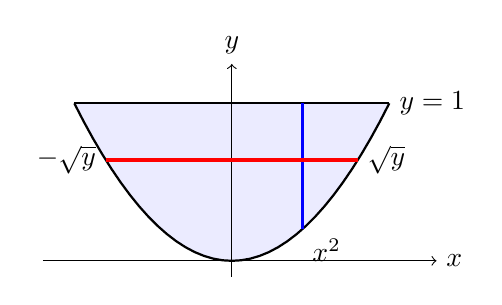
\begin{tikzpicture}[xscale=2,yscale=2]
\fill[blue!8] plot[domain=-1:1,samples=35] (\x,{\x*\x})--cycle;
\draw[thick] plot[domain=-1:1,samples=35] (\x,{\x*\x});
\draw[thick] (-1,1)--(1,1) node[right] {$y=1$};
\draw[->] (-1.2,0)--(1.3,0) node[right] {$x$};
\draw[->] (0,-.1)--(0,1.25) node[above] {$y$};
\draw[blue,very thick] (.45,.2025)--(.45,1);
\draw[red,very thick] (-.8,.64)--(.8,.64);
\node[left] at (-.8,.64) {$-\sqrt y$};\node[right] at (.8,.64) {$\sqrt y$};
\node[below right] at (.45,.2025) {$x^2$};
\end{tikzpicture}
\end{center}
The blue vertical slice starts at $x^2$; the red horizontal slice ends at
the two square roots. Consequently
\[
\operatorname{area}(E)=\int_{-1}^1(1-x^2)\,\dd x
=\int_0^1 2\sqrt y\,\dd y=\frac43.
\]
For a nonconstant integrand the same bounds give
$\int_E y=\int_0^1 2y^{3/2}\,\dd y=4/5$.
\end{minipage}
\end{example}

\begin{example}[The same triangle, two orders]
For $D=\{(x,y):0\leq x\leq1,\ 0\leq y\leq1-x\}$,
\[
\int_D x=\int_0^1\int_0^{1-x}x\,\dd y\,\dd x=\frac16
=\int_0^1\int_0^{1-y}x\,\dd x\,\dd y.
\]
Reversing the order means describing the same points with horizontal
sections; it does not mean merely exchanging two differential symbols.
\end{example}

\begin{example}[A triangular zero extension and a split order]
For $D=\{(x,y):0\leq x\leq1,\ 0\leq y\leq x\}$ and $f=x+y$,
the zero extension on $[0,1]^2$ has jumps only along the three boundary
segments. The graph-region theorem gives
\[
\int_D(x+y)=\int_0^1\int_0^x(x+y)\,\dd y\,\dd x
=\int_0^1\tfrac32x^2\,\dd x=\tfrac12.
\]
Reversing the order gives $\int_0^1\int_y^1(x+y)\,\dd x\,\dd y=1/2$.
For a region requiring a split, take
$E=\{(x,y):0\leq x\leq2,\ 0\leq y\leq\min(x,2-x)\}$.
Horizontal slices have $0\leq y\leq1$, $y\leq x\leq2-y$;
vertical slices require $[0,1]$ with upper edge $x$ and $[1,2]$
with upper edge $2-x$. Thus its area is both
\[
\int_0^1(2-2y)\,\dd y=1
\quad\text{and}\quad
\int_0^1x\,\dd x+\int_1^2(2-x)\,\dd x=1.
\]
The switch in the upper boundary at $x=1$ is why one iterated description
must be split.
\end{example}

\begin{center}
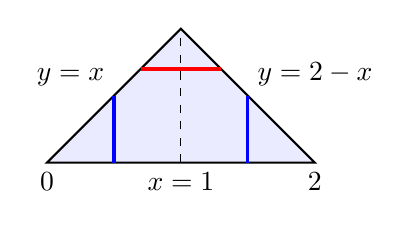
\begin{tikzpicture}[scale=1.7]
\fill[blue!8] (0,0)--(1,1)--(2,0)--cycle;
\draw[thick] (0,0)--(1,1)--(2,0)--cycle;
\draw[dashed] (1,0)--(1,1);
\draw[blue,very thick] (.5,0)--(.5,.5);
\draw[blue,very thick] (1.5,0)--(1.5,.5);
\draw[red,very thick] (.7,.7)--(1.3,.7);
\node[above left] at (.5,.5) {$y=x$};
\node[above right] at (1.5,.5) {$y=2-x$};
\node[below] at (1,0) {$x=1$};
\node[below] at (0,0) {$0$};\node[below] at (2,0) {$2$};
\end{tikzpicture}
\end{center}
In the preceding split-order example, vertical slices change their upper
edge at the dashed line; every horizontal slice has endpoints $y,2-y$.

\begin{lemma}[Lipschitz images of boxes and faces]
\label{lem:lipschitz-box-face}
If $F$ is $L$-Lipschitz on a subset of an $n$-cube of side $h$, its
image fits in a box of side $2L\sqrt n\,h$ (or is a singleton when
$L=0$). The image of a compact $(n-1)$-dimensional rectangular face
under a Lipschitz map into $\R^n$ is Jordan-null.
\end{lemma}
\begin{proof}
Choose one point of the subset. Every other point has distance at most
$\sqrt n h$ from it, so every image coordinate differs by at most
$L\sqrt n h$. This proves the box bound. Partition a face into at
most $C h^{-(n-1)}$ pieces of side at most $h$. The covering image
boxes have total volume at most $C(2L\sqrt n)^n h$, which tends to
zero. For $n=1$ a face is a point and a small interval covers its image.
The same argument handles a finite union of faces.
\end{proof}

\begin{theorem}[Lower-dimensional images cannot contain an open set]
\label{thm:lower-dimensional-image}
Let $f:U\subseteq\R^n\to\R^m$ be $C^1$ on an open set, with $n<m$.
The image of every closed cube $Q\subset U$ is compact and Jordan-null
in $\R^m$. The full image $f(U)$ has empty interior. Thus a map into a
nonempty open $V\subseteq\R^m$ cannot be surjective.
\end{theorem}
\begin{proof}
On $Q$, bound $\|Df\|$ by $L>0$. Its convexity makes $f|_Q$
$L$-Lipschitz. Subdivide a cube of side $s$ into $k^n$ cubes of side
$s/k$. Each image lies in an $m$-box of side $2L\sqrt n\,s/k$.
Their total $m$-volume is at most
\[
(2L\sqrt n\,s)^m k^{n-m}\longrightarrow0.
\]
Enlarging these finitely many boxes slightly makes them open while
keeping arbitrarily small total volume. Compactness of $f(Q)$ follows
from continuity. This proves the first assertion.

There are countably many closed cubes with rational center and positive
rational side length contained in $U$, and their interiors cover $U$:
a sufficiently small such cube around any point lies in an open ball
contained in $U$. Enumerate them as $Q_j$.
Suppose $f(U)$ contained a closed target cube $B$ of positive volume.
For a fixed $\varepsilon>0$, cover each $f(Q_j)$ by finitely many open
boxes of total volume less than $\varepsilon 2^{-j}$.
Together these form an open cover of the compact cube $B$, so finitely
many of the boxes cover $B$. Finite grid comparison then gives
$\operatorname{vol}(B)<\varepsilon$. Choosing
$\varepsilon<\operatorname{vol}(B)$ is a contradiction.
Every nonempty open set contains such a cube, proving empty interior.
For $n=0$ the source contains at most one point and the conclusion is immediate.
\end{proof}
This completes the deferred proof of \cref{thm:dimension-nonsurjective}.
The countable family was used only to construct an open cover of one
compact target cube and extract a finite subcover. No assertion that
$f(U)$ itself is Jordan-null, and no countable additivity of Jordan
content, is needed.

\subsection{Volumes in three dimensions by cross-sections}
Sketch the solid and choose a slicing direction. Describe a typical
two-dimensional cross-section by inequalities, then integrate its
contribution. Alternatively project onto the $xy$-plane
and write $z_-(x,y)\leq z\leq z_+(x,y)$; projections onto the $xz$- or
$yz$-plane instead describe intervals in $y$ or $x$.

\paragraph{What Fubini does for a solid.}
Let $\Omega$ lie between heights $a$ and $b$, and define its horizontal section
\[
\Omega_z=\{(x,y):(x,y,z)\in\Omega\},\qquad
A(z)=\int_{\Omega_z}1\,\dd(x,y).
\]
When $\Omega$ and all these sections are Jordan measurable, apply
\cref{lem:fubini-integrable-sections} to the zero-extended indicator:
\begin{align*}
\operatorname{vol}(\Omega)
&=\int_\Omega1\,\dd(x,y,z)\\
&=\int_a^b\left(\int_{\Omega_z}1\,\dd(x,y)\right)\dd z
=\int_a^b A(z)\,\dd z.
\end{align*}
Fixing $z$ leaves a planar region of admissible $(x,y)$ points. The inner
integral of $1$ gives its area; the outer integral accumulates those areas.

\paragraph{Checking the geometry needed by the theorem.}
For $R,h>0$, the cylinder and cone sides are images of $[0,2\pi]\times[0,h]$
under, respectively,
\begin{align*}
(\theta,z)&\longmapsto(R\cos\theta,R\sin\theta,z),\\
(\theta,z)&\longmapsto
\bigl(R(1-z/h)\cos\theta,R(1-z/h)\sin\theta,z\bigr).
\end{align*}
Their derivatives are bounded on these compact rectangles, so the maps
are Lipschitz. Their images are therefore Jordan-null by
\cref{lem:lipschitz-box-face}.
No regularity of the cone as a surface at its apex is needed for this argument.
The flat disk pieces lie in planes and are also null in three dimensions.
For the sphere use the six coordinate graph pieces where one coordinate
has magnitude at least $R/\sqrt3$; the corresponding square-root graphs
have bounded derivatives on their compact disk domains. The same covering
argument applies to these pieces. Thus each solid has Jordan-null boundary.
All horizontal sections are disks, whose circular boundaries are Lipschitz
images of an interval and hence null in the plane. The required indicators
and sections are therefore integrable.

The disk area used below follows from Cartesian slices and the one-variable
substitution $x=r\sin t$:
\[
\int_{-r}^r2\sqrt{r^2-x^2}\,\dd x
=2r^2\int_{-\pi/2}^{\pi/2}\cos^2t\,\dd t=\pi r^2.
\]
The case $r=0$ is zero. These examples do not presuppose polar change of variables.

\begin{example}[Cylinder and cone]\label{ex:cylinder-cone-slices}
Let $R,h>0$. For the cylinder
\[
C=\{(x,y,z):x^2+y^2\leq R^2,\ 0\leq z\leq h\},
\]
each height $z\in[0,h]$ gives the same section
$C_z=\{(x,y):x^2+y^2\leq R^2\}$. Its area is $A(z)=\pi R^2$.
The cross-sectional Fubini formula gives
\[
\operatorname{vol}(C)=\int_0^h A(z)\,\dd z
=\int_0^h\pi R^2\,\dd z=\pi R^2[z]_0^h=\pi R^2h.
\]
Thus ``base area times height'' is itself an iterated-integral calculation.

For the cone
\[
K=\{(x,y,z):0\leq z\leq h,\ x^2+y^2\leq R^2(1-z/h)^2\},
\]
fixing $z$ leaves a disk with radius $r(z)=R(1-z/h)$, since $1-z/h\geq0$.
Consequently
\[
A(z)=\pi r(z)^2=\pi R^2(1-z/h)^2.
\]
The radius decreases linearly with height, so area decreases quadratically.
Integrating this quadratic profile is what produces the factor $1/3$:
\begin{align*}
\operatorname{vol}(K)
&=\int_0^h\pi R^2(1-z/h)^2\,\dd z\\
&=\pi R^2\int_0^h\left(1-\frac{2z}{h}+\frac{z^2}{h^2}\right)\dd z\\
&=\pi R^2\left[z-\frac{z^2}{h}+\frac{z^3}{3h^2}\right]_0^h\\
&=\pi R^2(h-h+h/3)=\frac13\pi R^2h.
\end{align*}
Compared with the cylinder of the same base and height, the cone has one
third of the volume because its sections shrink according to this profile.
\begin{center}
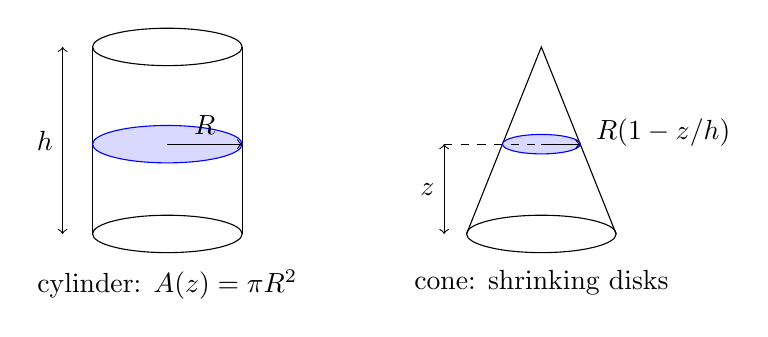
\begin{tikzpicture}[scale=.95]
\draw (-1,0)--(-1,2.5) (1,0)--(1,2.5);
\draw (0,0) ellipse (1 and .25);\draw (0,2.5) ellipse (1 and .25);
\filldraw[fill=blue!15,draw=blue] (0,1.2) ellipse (1 and .25);
\draw[->] (0,1.2)--(1,1.2) node[midway,above] {$R$};
\draw[<->] (-1.4,0)--(-1.4,2.5) node[midway,left] {$h$};
\node[below] at (0,-.35) {cylinder: $A(z)=\pi R^2$};
\begin{scope}[xshift=5cm]
\draw (-1,0)--(0,2.5)--(1,0);\draw (0,0) ellipse (1 and .25);
\filldraw[fill=blue!15,draw=blue] (0,1.2) ellipse (.52 and .13);
\draw[->] (0,1.2)--(.52,1.2);
\node[right] at (.6,1.35) {$R(1-z/h)$};
\draw[dashed] (-1.3,1.2)--(0,1.2);
\draw[<->] (-1.3,0)--(-1.3,1.2) node[midway,left] {$z$};
\node[below] at (0,-.35) {cone: shrinking disks};
\end{scope}
\end{tikzpicture}
\end{center}
\end{example}
\begin{example}[A ball from horizontal disks]\label{ex:ball-slices}
For $B_R=\{(x,y,z):x^2+y^2+z^2\leq R^2\}$, the height range is $[-R,R]$.
At a fixed height,
\[
(B_R)_z=\{(x,y):x^2+y^2\leq R^2-z^2\},\qquad
A(z)=\pi(R^2-z^2).
\]
The radius is $\sqrt{R^2-z^2}$, zero at the poles and $R$ at the equator.
Applying the same cross-sectional formula gives
\begin{align*}
\operatorname{vol}(B_R)
&=\int_{-R}^R\pi(R^2-z^2)\,\dd z
=\pi\left[R^2z-\frac{z^3}{3}\right]_{-R}^R\\
&=\pi\left(\frac23R^3-\left(-\frac23R^3\right)\right)
=\frac43\pi R^3.
\end{align*}
This is a genuine triple integral reduced to one variable by first
understanding the geometry and area of every two-dimensional section.

\noindent\begin{minipage}{\linewidth}
\begin{center}
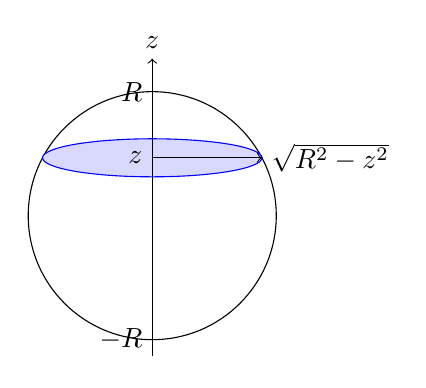
\begin{tikzpicture}[scale=1.05]
\draw (0,0) circle(1.5);
\filldraw[fill=blue!15,draw=blue] (0,.7) ellipse (1.327 and .23);
\draw[->] (0,-1.7)--(0,1.9) node[above] {$z$};
\draw[->] (0,.7)--(1.327,.7) node[right] {$\sqrt{R^2-z^2}$};
\node[left] at (0,1.5) {$R$};\node[left] at (0,-1.5) {$-R$};
\node[left] at (0,.7) {$z$};
\end{tikzpicture}
\end{center}
Once the disk geometry is understood, the three-dimensional calculation
reduces to an elementary one-variable integral.
\end{minipage}
\end{example}

\section{Linear Changes of Variables}

The one-variable substitution rule says that $\abs{\phi'(t)}$ measures the
local stretching of length.  In several variables, the corresponding linear
fact comes first: an invertible linear map $L$ sends a small box to a
parallelepiped and scales its volume by $\abs{\det L}$.  A coordinate scaling
by $c$ has factor $\abs c$, a diagonal map has the product of its coordinate
scalings, a shear has factor $1$, and a coordinate reflection preserves volume.
Thus the determinant is the natural volume-scaling number, not a formal
correction inserted after the fact.

\begin{example}[A rectangle becomes a parallelogram]
Let
\[
L(s,t)=(2s+t,s+3t).
\]
The unit square is sent to the parallelogram spanned by $(2,1)$ and $(1,3)$.
Since
\[
\det L=\det\begin{pmatrix}2&1\\1&3\end{pmatrix}=5,
\]
its area is $5$.  More generally, the image of a rectangle of area $A$ has
area $5A$.  The linear change-of-variables theorem below turns this geometric
calculation into an integral formula.
\end{example}

\begin{lemma}[Volume under an invertible linear map]
\label{lem:linear-volume}
Let
\[
L:\R^n\longrightarrow\R^n
\]
be invertible and let $Q$ be a rectangle.  Then $L(Q)$ is Jordan measurable
and
\[
\operatorname{vol}(L(Q))
=\abs{\det L}\operatorname{vol}(Q).
\]
More generally, if \(E\subseteq\R^n\) is Jordan measurable, then \(L(E)\)
is Jordan measurable and
\[
\operatorname{vol}(L(E))
=\abs{\det L}\operatorname{vol}(E).
\]
\end{lemma}
\begin{proof}
We first record the effect of the three simple invertible linear maps on
Jordan volume. If a rectangle has a zero side length, it lies in a
rectangular face. Its image under any linear map is Jordan-null by
\cref{lem:lipschitz-box-face}, since linear maps are Lipschitz. Both
volumes are then zero. For the rectangle calculations below assume all
side lengths are positive. A coordinate permutation merely permutes the side intervals
of a rectangle and preserves its volume.  Multiplication of one coordinate
by \(c\ne0\) takes a rectangle to a rectangle and multiplies its volume by
\(\abs c\).

\textbf{Strategy for a shear.} A shear translates every fiber without
changing its length; first prove Jordan measurability, then apply Fubini.
After relabeling coordinates, write $R=A\times[a,b]$ and
$S(z,t)=(z,t+cz_j)$. As $S$ is a homeomorphism,
$\partial S(R)=S(\partial R)$. The boundary of $R$ is a finite union
of rectangular faces, whose Lipschitz images are Jordan-null by
\cref{lem:lipschitz-box-face}. The boundary criterion
(\cref{prop:jordan-boundary-criterion}) therefore proves that $S(R)$
is Jordan measurable before Fubini is invoked.
Choose a compact interval $J$ containing all translated fibers.
For each $z\in A$, the fiber is $[a+cz_j,b+cz_j]$, so
\[
\int_J\mathbf1_{S(R)}(z,t)\,\dd t=b-a.
\]
All these sections are integrable. By \cref{lem:fubini-integrable-sections},
\[
\operatorname{vol}(S(R))
=\int_A\left(\int_J\mathbf1_{S(R)}(z,t)\,\dd t\right)\dd z
=(b-a)\operatorname{vol}(A)=\operatorname{vol}(R).
\]

These conclusions extend from rectangles to every Jordan-measurable set.
Indeed, for such a set \(E\), the Darboux criterion applied to
\(\mathbf1_E\) gives finite unions \(I\) and \(O\) of grid rectangles with
pairwise disjoint interiors such that
\[
I\subseteq E\subseteq O,
\qquad
\operatorname{vol}(O)-\operatorname{vol}(I)<\varepsilon.
\]
Images of distinct grid rectangles under a simple map overlap only in
images of their common faces. By \cref{lem:lipschitz-box-face},
those images are Jordan-null.
Thus these overlaps are Jordan-null, and
\cref{prop:jordan-null-additivity} shows that the volumes of the images of
\(I\) and \(O\) are the sums of the volumes of their pieces.  The inclusions
\[
S(I)\subseteq S(E)\subseteq S(O)
\]
then make the upper and lower Jordan integrals of \(\mathbf1_{S(E)}\) differ
by less than \(\varepsilon\).  The same argument applies to coordinate
permutations and coordinate scalings.  Consequently, each of these simple maps
sends Jordan-measurable sets to Jordan-measurable sets and multiplies their
volumes by the absolute value of its determinant.

\Cref{lem:elementary-factorization} gives geometric maps $G_1,\ldots,G_k$
with $L=G_k\circ\cdots\circ G_1$, each a permutation, scaling, or shear.
The rightmost map acts first. Start with $A_0=E$ and put
$A_j=G_j(A_{j-1})$ for $j=1,\ldots,k$. The result just proved first
makes $A_j$ Jordan measurable and then gives
\[
\operatorname{vol}(A_j)=|\det G_j|\operatorname{vol}(A_{j-1}).
\]
Thus $A_k=L(E)$ is Jordan measurable before its volume is used. Multiplying
these finite identities in their order of application gives
\[
\operatorname{vol}(L(E))=\left(\prod_{j=1}^k|\det G_j|\right)
\operatorname{vol}(E)=|\det L|\operatorname{vol}(E).
\]
For $L=I$ the empty composition has factor $1$.
Taking $E=[0,1]^n$ gives volume $|\det L|$; taking $E=Q$ gives the
rectangle assertion directly, including degenerate rectangles.

For completeness, measurability can also be read directly from the boundary.
Since \(L\) is a homeomorphism,
\[
\partial L(Q)=L(\partial Q).
\]
Each face of \(Q\) can be covered by at most \(C_0h^{-(n-1)}\) face-cubes of
side at most \(h\).  If \(M=\norm L_{\mathrm{op}}\), the image of each such
piece has diameter at most \(M\sqrt n\,h\), and hence lies in an
axis-parallel \(n\)-box of side \(2M\sqrt n\,h\).  The total volume of these
boxes is at most
\[
C_0(2M\sqrt n)^nh,
\]
which tends to zero.  A finite union over the faces proves that
\(\partial L(Q)\) is Jordan-null, in agreement with
\cref{prop:jordan-boundary-criterion}.
\end{proof}

\begin{theorem}[Linear change of variables]
\label{thm:linear-change-variables}
Let $L:\R^n\to\R^n$ be invertible, let $E$ be Jordan measurable, and let
\[
f:L(E)\longrightarrow\R
\]
have an integrable zero extension.  Then $L(E)$ is Jordan measurable and
\[
\int_{L(E)}f(y)\,\dd y
=
\int_Ef(Lx)\abs{\det L}\,\dd x.
\]
\end{theorem}
\begin{proof}
Let \(R\) be a rectangle and let
\[
s=\sum_{i=1}^{N}c_i\mathbf1_{R_i}
\]
be a finite sum for the closed cells of a grid partition of \(R\).
On shared faces this formula sums all incident terms. This is harmless for
its integral, but we do not use those values as pointwise bounds for another
function. This enlarges the initial owned-cell convention: arbitrary bounded values
on the finitely many grid faces change no integral by the established
null-modification result. More generally we call a bounded function a grid step function
if it is constant on each cell interior, allowing arbitrary bounded values
on the union $G$ of grid faces. Such a function differs from the displayed
sum only on the Jordan-null set $G$, so has the same integral by
\cref{prop:jordan-null-additivity}. Its transform differs only on $L(G)$,
also Jordan-null by \cref{lem:lipschitz-box-face}.
The sets \(L(R_i)\) are Jordan measurable by
\cref{lem:linear-volume}.  Two of them intersect only in the image of a
common grid face, which is Jordan-null by \cref{lem:lipschitz-box-face}.  Hence \cref{prop:jordan-null-additivity} gives
\[
\int_{L(R)}s(L^{-1}y)\,\dd y
=
\sum_{i=1}^{N}c_i\operatorname{vol}(L(R_i))
=
\abs{\det L}\int_Rs(x)\,\dd x.
\]
Thus the formula is established first for rectangular step functions; their
transforms are finite sums of indicators of the Jordan sets \(L(R_i)\),
not rectangular step functions in the \(y\)-coordinates.

Now let \(h:R\to\R\) be Riemann integrable.  For every \(\varepsilon>0\),
choose a grid whose Darboux gap is less than $\varepsilon$.
On the interior of its cell $R_i$, put
$\ell=\inf_{R_i}h$ and $u=\sup_{R_i}h$.
On the entire face set $G$, instead put $\ell=-M$ and $u=M$, where
$M\geq\sup_R|h|$. These are grid step functions in the preceding sense.
The bounds now hold even on shared and exterior faces. Null modification
leaves their integrals equal to the lower and upper Darboux sums, so
\[
\ell\leq h\leq u,
\qquad
\int_R(u-\ell)<\varepsilon.
\]
Their transforms are integrable on \(L(R)\), and
\[
\ell(L^{-1}y)\leq h(L^{-1}y)\leq u(L^{-1}y).
\]
The gap between the transformed upper and lower integrals is
\[
\abs{\det L}\int_R(u-\ell)
<
\abs{\det L}\varepsilon.
\]
To make the integrability conclusion explicit, choose Darboux partitions for
the two transformed integrable step functions whose upper--lower gaps have
sum less than an arbitrary \(\delta>0\), and pass to a common refinement.
On that refinement, the upper sum of \(h\circ L^{-1}\) is at most the upper
sum of \(u\circ L^{-1}\), while its lower sum is at least the lower sum of
\(\ell\circ L^{-1}\).  Its Darboux gap is consequently less than
\[
\abs{\det L}\varepsilon+\delta.
\]
Since \(\varepsilon\) and \(\delta\) are arbitrary,
\(h\circ L^{-1}\) is integrable on \(L(R)\).  Squeezing its integral between
the two transformed step-function integrals proves
\[
\int_{L(R)}h(L^{-1}y)\,\dd y
=
\abs{\det L}\int_Rh(x)\,\dd x.
\]
All integrations here may be read through zero extensions to containing
rectangles, as in the definition of integration over a Jordan set.

Apply the same lower--upper construction to \(\mathbf1_E\) on a rectangle
containing \(E\).  The transformed indicators squeeze
\(\mathbf1_{L(E)}\), with integral gap multiplied by \(\abs{\det L}\).
Hence \(L(E)\) is Jordan measurable before any integral over it is used.

Finally, choose a rectangle \(P\) containing \(L(E)\), and let
\(\widetilde f\) be the integrable zero extension of \(f\) to \(P\).
Apply the preceding argument to \(L^{-1}\) and \(\widetilde f\).  It proves
that
\[
x\longmapsto\widetilde f(Lx)
\]
has an integrable zero extension from \(L^{-1}(P)\), and
\[
\int_P\widetilde f(y)\,\dd y
=
\abs{\det L}\int_{L^{-1}(P)}\widetilde f(Lx)\,\dd x.
\]
The integrands vanish, respectively, outside \(L(E)\) and outside \(E\).
Using the definition of integration over Jordan sets therefore turns this
identity into the asserted formula.
\end{proof}


\Needspace{19\baselineskip}
\begin{example}[An ellipse and an ellipsoid by scaling]\label{ex:ellipse-scaling}
Let $a,b,c>0$. The map $\sigma(u,v)=(au,bv)$ takes the unit disk $D$
onto $E=\{x^2/a^2+y^2/b^2\leq1\}$. Its derivative is
$\operatorname{diag}(a,b)$, so $|\det D\sigma|=ab$ and
$\operatorname{area}(E)=ab\operatorname{area}(D)=\pi ab$.
\begin{center}
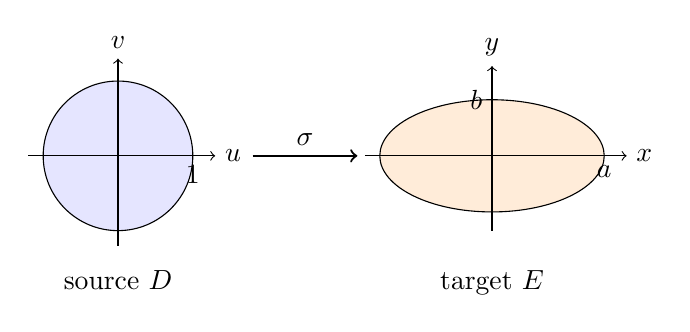
\begin{tikzpicture}[scale=.95]
\filldraw[fill=blue!10] (0,0) circle(1);
\draw[->] (-1.2,0)--(1.3,0) node[right] {$u$};
\draw[->] (0,-1.2)--(0,1.3) node[above] {$v$};
\draw[->,thick] (1.8,0)--(3.2,0) node[midway,above] {$\sigma$};
\filldraw[fill=orange!15] (5,0) ellipse(1.5 and .75);
\draw[->] (3.3,0)--(6.8,0) node[right] {$x$};
\draw[->] (5,-1)--(5,1.2) node[above] {$y$};
\node[below] at (1,0) {$1$};\node[below] at (6.5,0) {$a$};
\node[left] at (5,.75) {$b$};
\node[below] at (0,-1.4) {source $D$};\node[below] at (5,-1.4) {target $E$};
\end{tikzpicture}
\end{center}
Likewise $(u,v,w)\mapsto(au,bv,cw)$ has determinant $abc$ and takes
the unit ball to $x^2/a^2+y^2/b^2+z^2/c^2\leq1$. Hence the ellipsoid
volume is $4\pi abc/3$. Slicing found the ball's volume; linear scaling
now transfers it to a new solid.
\end{example}

\section{Nonlinear Changes of Variables}
\label{sec:nonlinear-change}
The local structure from Chapter~11 turns a multivariable substitution
into one-variable substitutions with parameters. Our main route is
\[
\boxed{\text{primitive}\ \longrightarrow\ \text{composition}\
\longrightarrow\ \text{local}\ \longrightarrow\ \text{finite localization}.}
\]
Jordan boundaries will be handled separately after the integral identity.
The determinant measures local volume distortion, but establishing that
geometric interpretation need not precede the structural proof.

\subsection{Primitive substitution and composition}
For a continuous function $f$ on an open set $V$, write $f\in C_c(V)$
if its support in $V$ is compact. Recall that support is the closure of
the nonzero set (\cref{def:euclidean-function-support}). Such a support has positive distance
from the complement of $V$ when that complement is nonempty: finitely
many doubled balls inside $V$ cover it by their smaller balls. Therefore
zero extension of $f$ is continuous on $\R^n$. Its integral over $V$
means the ordinary Riemann integral of that extension on any rectangle
containing its support in the interior. Restriction and gluing show
independence of this rectangle. No improper integral is being introduced.

\begin{lemma}[Primitive change of variables]\label{lem:primitive-substitution}
Let $q:U\to V$ be a primitive $C^1$ diffeomorphism of open sets.
For every $f\in C_c(V)$,
\[
\int_V f(y)\,\dd y=\int_U f(q(x))|\det Dq(x)|\,\dd x.
\]
\end{lemma}
\begin{proof}
First suppose the changed coordinate is the last one, so
$q(x',t)=(x',p(x',t))$ and $\det Dq=\partial_t p$.
Both $f$ and $g=(f\circ q)|\partial_t p|$ have continuous zero
extensions with compact support: the support of $g$ is contained in
$q^{-1}(\operatorname{supp}f)$, which is compact by continuity of $q^{-1}$.
Choose enclosing rectangles for these two supports.

Fix $x'$. The source slice $U_{x'}=\{t:(x',t)\in U\}$ is open in
$\R$, and its components are open intervals. On each such interval
$\partial_t p$ is continuous and never zero, so has constant sign;
the mean value theorem makes $p(x',\cdot)$ strictly monotone there.
Injectivity of $q$ makes the images of distinct component intervals
disjoint, and surjectivity onto $V$ makes their union $V_{x'}$.

Only finitely many of these intervals meet the compact slice of
$q^{-1}(\operatorname{supp}f)$. Indeed, every point of that slice has
an interval neighborhood contained in $U_{x'}$, and a finite subcover
meets only finitely many components. Within each relevant component
choose a closed subinterval $[\alpha,\beta]$ with that component's
compact support slice in its interior. Define
\[
\begin{aligned}
s_-&=\min\{p(x',\alpha),p(x',\beta)\},\\
s_+&=\max\{p(x',\alpha),p(x',\beta)\}.
\end{aligned}
\]
One-variable substitution, \cref{thm:one-variable-substitution}, gives
\[
\int_\alpha^\beta f(x',p(x',t))|\partial_t p(x',t)|\,\dd t
=\int_{s_-}^{s_+}f(x',s)\,\dd s.
\]
For an increasing fiber map this is substitution directly. For a
decreasing map, $|\partial_t p|=-\partial_t p$; the negative sign
reverses the endpoint order in the substituted integral. The minimum
and maximum therefore give the same formula in both cases.
Outside these finitely many subintervals and their images the slice
integrands are zero.
Adding yields equality of the integrals of the full zero-extended slices.
This uses only finitely many ordinary interval integrals for each $x'$,
even if the open domain has infinitely many slice components.
Fubini for the continuous zero extensions now integrates that equality
over $x'$. For $n=1$ there are no parameter coordinates. Any other
changed coordinate is moved to the last position by coordinate
permutations, which preserve integrals by Fubini and have absolute
determinant one.
\end{proof}
Thus a primitive multivariable substitution is ordinary one-variable
substitution with parameters. The absolute value accounts for decreasing
fibers as well as increasing ones.

\begin{lemma}[Stability under composition]\label{lem:substitution-composition}
Suppose the compact-support formula holds for $C^1$ diffeomorphisms
$\sigma:U\to V$ and $\tau:V\to W$. It then holds for $\tau\circ\sigma$.
It also holds for restrictions of any such map to open subsets.
\end{lemma}
\begin{proof}
For $f\in C_c(W)$ the function $h=(f\circ\tau)|\det D\tau|$ lies
in $C_c(V)$, since its support lies in the compact set
$\tau^{-1}(\operatorname{supp}f)$. Applying the two formulas gives
\[
\begin{aligned}
\int_W f
 &=\int_V(f\circ\tau)|\det D\tau|\\
 &=\int_U(f\circ\tau\circ\sigma)
       |\det D\tau(\sigma(x))|\,|\det D\sigma(x)|\,\dd x.
\end{aligned}
\]
The chain rule and multiplicativity of the determinant identify the
product as $|\det D(\tau\circ\sigma)(x)|$.
For a restriction $\sigma|_{U_0}$, $U_0\subset U$ open, extend a function in
$C_c(\sigma(U_0))$ by zero to $V$ and use the original formula. Its
pullback vanishes outside $U_0$, giving exactly the restricted identity.
\end{proof}

\begin{corollary}[Local change of variables]\label{cor:local-structural-change}
If $D\sigma(a)$ is invertible for a $C^1$ map $\sigma$ on an open set,
there is a neighborhood $N$ of $a$ on which the compact-support
change-of-variables formula holds for $\sigma:N\to\sigma(N)$.
\end{corollary}
\begin{proof}
Use \cref{thm:primitive-factorization}. Each primitive factor satisfies
\cref{lem:primitive-substitution}; coordinate permutations satisfy the
formula by Fubini, with absolute determinant one. Successive applications
of \cref{lem:substitution-composition} give the assertion.
\end{proof}

\subsection{The compact-support theorem}
\begin{theorem}[Change of variables on open sets with compact support]
\label{cor:compact-support-change-variables}
Let $\sigma:U\to V$ be a $C^1$ diffeomorphism between open subsets of
$\R^n$. For every $f\in C_c(V)$,
\[
\boxed{\int_V f(y)\,\dd y
=\int_U f(\sigma(x))|\det D\sigma(x)|\,\dd x.}
\]
If $\det D\sigma>0$ the absolute value may be omitted. If it is negative
everywhere, omitting it reverses the sign.
\end{theorem}
\begin{proof}
Let $K=\operatorname{supp}f$ and $L=\sigma^{-1}(K)$. The latter set is
compact as the continuous image of $K$ under $\sigma^{-1}$.
If $K$ is empty the identity is zero equals zero. Otherwise cover $L$
by finitely many neighborhoods $N_i\subset U$ from
\cref{cor:local-structural-change}. Choose the finite Euclidean weights
$\rho_i$ of \cref{thm:finite-euclidean-pou}, compactly supported in
$N_i$, with sum one near $L$. On $\sigma(N_i)$ put
\[
f_i(y)=\rho_i(\sigma^{-1}(y))f(y).
\]
Its support is contained in the compact subset
$\sigma(\operatorname{supp}\rho_i)\subset\sigma(N_i)$, so $f_i$ belongs
to $C_c(\sigma(N_i))$ and extends continuously by zero to $V$.
Where $f(y)\ne0$, $\sigma^{-1}(y)\in L$ and the weights sum to one;
where $f(y)=0$, all $f_i$ vanish. Thus $\sum_i f_i=f$ on $V$.
The local formula says
\[
\int_{\sigma(N_i)}f_i
=\int_{N_i}\rho_i(x)f(\sigma(x))|\det D\sigma(x)|\,\dd x.
\]
All these functions have compact support in their displayed domains.
Their zero extensions permit a finite sum on containing rectangles.
On $U$ the sum of the source integrands is
$f(\sigma(x))|\det D\sigma(x)|$, because that function vanishes outside
$L$. Summing gives the claimed formula. The sign assertions follow
from the absolute determinant.
\end{proof}

\subsection{Jordan boundaries and compact regions}
The preceding theorem establishes an integral identity for continuous
compactly supported functions. The next estimate supplies the separate
set-theoretic fact needed to integrate on compact Jordan regions.

\begin{lemma}[$C^1$ maps preserve compact Jordan-null sets]
\label{lem:c1-jordan-null}
Let $\sigma:U\subseteq\R^n\to\R^n$ be $C^1$, with $U$ open.
The image of a compact Jordan-null set $A\subset U$ is Jordan-null.
If $\sigma:U\to V$ is a diffeomorphism and $E\subset U$ is compact
and Jordan measurable, then $\sigma(E)$ is Jordan measurable and
$\partial\sigma(E)=\sigma(\partial E)$.
\end{lemma}
\begin{proof}
Choose $\delta>0$ so that the closed $\delta$-neighborhood of $A$
is compact in $U$, using a finite cover by doubled balls in $U$.
Bound $\|D\sigma\|$ there by a positive constant $L$. Each cube of
diameter less than $\delta$ meeting $A$ lies in that neighborhood.
Segments in that cube remain there, so the mean-value estimate bounds
image distances by $L$ times source distances. A cube of side $h$ maps
into a box of side $2L\sqrt n\,h$ by \cref{lem:lipschitz-box-face}.

For any $\varepsilon>0$, cover $A$ by finitely many open boxes of
total volume below $\varepsilon$. Their union contains a positive
neighborhood of $A$ by compactness. A sufficiently fine grid has all
cells meeting $A$ inside that union; their total volume is at most
$\varepsilon$ by finite grid comparison. Their image boxes have total
volume at most $(2L\sqrt n)^n\varepsilon$. This proves nullity.
A homeomorphism of open sets preserves relative boundary. The compact
sets $E,\sigma(E)$ lie inside their respective open domains, so their
relative and ambient boundaries coincide. Consequently
$\partial\sigma(E)=\sigma(\partial E)$ is null, and the Jordan boundary
criterion proves the final assertion.
\end{proof}

\begin{corollary}[Change of variables for compact Jordan regions]
\label{cor:jordan-nonlinear-change}
Let $\sigma:U\to V$ be a $C^1$ diffeomorphism of open sets,
$E\subset U$ compact and Jordan measurable, and $f$ continuous on
$\sigma(E)$. Then
\[
\int_{\sigma(E)}f=\int_E f(\sigma(x))|\det D\sigma(x)|\,\dd x.
\]
\end{corollary}
\begin{proof}
Both regions are Jordan measurable by \cref{lem:c1-jordan-null}.
Put $M=\max_{\sigma(E)}|f|$ and $J_0=\max_E|\det D\sigma|$;
the empty case is immediate. Fine-grid cells meeting $\partial E$
have total volume $v_h\to0$. Work in a fixed compact neighborhood of
$E$ inside $U$ and bound $\|D\sigma\|$ there by $L>0$.
The image of any union of these small cells has outer volume at most
$Cv_h$, $C=(2L\sqrt n)^n$, by the preceding cube estimate.

Let $O_h$ be a bounded open union of slightly enlarged boundary cells.
The enlargements can be chosen so their total volume is at most $2v_h$,
all stay in the fixed neighborhood, and their image boxes have total
volume at most $2Cv_h$. The set $K_h=E\setminus O_h$ is compact in
$E^\circ$. Choose $\eta_h\in C_c^\infty(E^\circ)$ equal to one near
$K_h$, with values in $[0,1]$. Define on $V$
\[
f_h(y)=
\begin{cases}
\eta_h(\sigma^{-1}(y))f(y),&y\in\sigma(E),\\
0,&y\notin\sigma(E).
\end{cases}
\]
Although $f$ is given only on $\sigma(E)$, this extension is continuous:
the cutoff has compact support in $E^\circ$ and vanishes near the
boundary. Its image support is compact in $\sigma(E^\circ)$, so
$f_h\in C_c(V)$. Apply \cref{cor:compact-support-change-variables}.
The source and target errors are confined to $E\cap O_h$ and its
image, respectively. All involved restricted integrands are integrable
by the compact Jordan theory, and domination by the finite box covers
gives
\[
\left|\int_{\sigma(E)}f-\int_V f_h\right|\leq2MCv_h,
\qquad
\left|\int_E(f\circ\sigma)|\det D\sigma|
-\int_E\eta_h(f\circ\sigma)|\det D\sigma|\right|\leq2MJ_0v_h.
\]
Letting the grid size tend to zero proves the assertion. No extension
of $f$ beyond its given region has been assumed.
\end{proof}

\begin{theorem}[Change of variables on a rectangle]\label{thm:change-of-variables}
Let $Q\subseteq\R^n$ be a rectangle, $U$ an open neighborhood of $Q$,
and $\sigma:U\to\R^n$ be $C^1$. Suppose $\sigma$ is injective on $Q$
and $\det D\sigma(x)\ne0$ for $x\in Q$. Then $\sigma(Q)$ is Jordan
measurable and, for continuous $f$ on $\sigma(Q)$,
\[
\int_{\sigma(Q)}f(y)\,\dd y
=\int_Q f(\sigma(x))|\det D\sigma(x)|\,\dd x.
\]
\end{theorem}
\begin{proof}
There is an open neighborhood of $Q$ on which $\sigma$ is injective.
Otherwise, in neighborhoods of distance less than $1/j$ from $Q$
inside a fixed compact neighborhood in $U$, there would be distinct
$x_j,y_j$ with $\sigma(x_j)=\sigma(y_j)$. Subsequences converge to
$x,y\in Q$. Continuity and injectivity on $Q$ give $x=y$.
The inverse theorem gives a neighborhood of this common limit where
$\sigma$ is injective; eventually both sequences lie there, a contradiction.
Continuity of the determinant and compactness also give a neighborhood
of $Q$ where it never vanishes. On the intersection $\sigma$ is an
injective local diffeomorphism, hence a diffeomorphism onto an open image:
the local smooth inverses agree by injectivity. Apply
\cref{cor:jordan-nonlinear-change} with $E=Q$.
\end{proof}

\subsection{Optional geometric refinement: local volume distortion}
The structural proof is complete. The following independent local
comparison retains the geometric insight of a direct Riemann proof.
Its inner estimate uses the inverse already supplied by Chapter~11.

\paragraph{The maximum-norm segment estimate.}
Let $H:\Omega\subseteq\R^n\to\R^m$ be differentiable on an open
neighborhood of $[x,y]$ and suppose
$\|DH(z)\|_{\infty\to\infty}\leq M$ along that segment.
Choose a coordinate $i$ with
$|H_i(y)-H_i(x)|=\|H(y)-H(x)\|_\infty$.
The scalar mean value theorem applied to
$t\mapsto H_i(x+t(y-x))$ on $[0,1]$ gives some $z\in[x,y]$ with
\[
\begin{aligned}
\|H(y)-H(x)\|_\infty
&=|DH_i(z)(y-x)|\\
&\leq\|DH(z)(y-x)\|_\infty
\leq M\|y-x\|_\infty.
\end{aligned}
\]
For $x=y$ the conclusion is immediate. In particular the estimate applies
on a convex region with this derivative bound, with the exact same constant.

\begin{proposition}[Local Jacobian volume distortion]\label{lem:local-volume-comparison}
Let $\sigma$ be $C^1$ near $a$, with $D\sigma(a)$ invertible. For every
$\varepsilon>0$ there is a neighborhood $N$ of $a$ such that every
nondegenerate closed cube $C\subset N$ satisfies
\[
\left|\frac{\operatorname{vol}\sigma(C)}{\operatorname{vol}C}
-|\det D\sigma(a)|\right|<\varepsilon.
\]
In particular this ratio tends to $|\det D\sigma(a)|$ as the cubes
shrink to $a$.
\end{proposition}
\begin{proof}
Put $A=D\sigma(a)$ and $T(x)=a+A^{-1}(\sigma(x)-\sigma(a))$.
Then $T(a)=a$, $DT(a)=I$, and the inverse theorem provides a local
inverse $S$ with $DS(a)=I$. Use the maximum norm and its operator norm.
Choose a convex ball about $a$ in the source and a convex ball about
$a$ in the image on which respectively
\[
\|DT-I\|_{\mathrm{op}}\leq\delta,
\qquad \|DS-I\|_{\mathrm{op}}\leq\delta,
\qquad 0<\delta<1.
\]
Continuity of $DT,DS$ allows this for any $\delta>0$.
Shrink $N$ so that cubes $C\subset N$ stay in the source ball and
all points within their half side length of $T(c)$ stay in the image
ball, where $c$ is the cube center. Concretely, if the image ball has
radius $R$, take $N=B_\infty(a,r)$ with $r<R/4$, inside the source
ball, and $T(N)\subset B_\infty(a,R/2)$. A cube in $N$ has side
$h\leq2r$, so these target points lie in $B_\infty(a,3R/4)$.
The maximum-norm segment estimate just proved, applied to $T-I$ and
$S-I$ on their respective convex balls, gives
\[
\|T(x)-T(c)-(x-c)\|_\infty\leq\delta\|x-c\|_\infty
\qquad(x\in C).
\]
Thus $T(C)$ lies in the cube centered at $T(c)$ of side $(1+\delta)h$.
Conversely, if $\|y-T(c)\|_\infty\leq h/(2(1+\delta))$, the segment
from $T(c)$ to $y$ is in the chosen image ball and
\[
\|S(y)-c\|_\infty\leq(1+\delta)\|y-T(c)\|_\infty\leq h/2.
\]
So the cube of side $h/(1+\delta)$ about $T(c)$ lies in $T(C)$.
The image is Jordan measurable by \cref{lem:c1-jordan-null}, independently
of the integral formula. Monotonicity of volume and linear volume scaling yield
\[
|\det A|(1+\delta)^{-n}
\leq\frac{\operatorname{vol}\sigma(C)}{\operatorname{vol}C}
\leq|\det A|(1+\delta)^n.
\]
Choose $\delta$ so that both endpoints differ from $|\det A|$ by less
than $\varepsilon$. This proves the uniform neighborhood assertion.
\end{proof}

\paragraph{Schwartz's 1954 perspective.}
An alternative direct Riemann/Jordan proof is Schwartz's
\cite{schwartz-change}. Its reusable principle is to obtain the easy
one-sided volume or integral bound from local derivative estimates,
then apply that bound to the inverse map. For example, once the upper
bound $\int_{\sigma(E)}q\leq\int_E(q\circ\sigma)J_\sigma$ is known for
nonnegative continuous $q$, apply it to $\sigma^{-1}$ and
$h=(q\circ\sigma)J_\sigma$. Since
$J_{\sigma^{-1}}(\sigma(x))J_\sigma(x)=1$, this gives the reverse inequality.
This avoids solving a hard inner-containment problem directly:
\[
\boxed{\text{one inequality for }\sigma
+\text{the same inequality for }\sigma^{-1}
\ \Longrightarrow\ \text{equality}.}
\]
This is a proof perspective, not a second full proof. The local geometric
viewpoint can also be compared with \cite{pugh-analysis,bartle-elements}.

\paragraph{Lebesgue perspective (unproved preview).}
In Lebesgue theory the theorem first describes transformed measure:
\[
m(\sigma(E))=\int_E |\det D\sigma(x)|\,\dd x
\]
for measurable $E\subset U$. More precisely, the measure on $U$ defined
by $\nu(E)=m(\sigma(E))$ is $(\sigma^{-1})_*m|_V$; its Radon--Nikodym
density relative to $m|_U$ is $|\det D\sigma|$. Integration with respect
to this transformed measure gives the function formula, first for
nonnegative measurable functions and then for integrable ones. The
present Riemann/Jordan proof uses finite smooth localization; Lebesgue
theory permits measurable localization and countable additivity.
These measure-theoretic statements are a non-prerequisite preview,
not results proved here; see \cite{knapp-basic-real}.

\begin{lemma}[Derivatives on half-space domains]\label{lem:halfspace-derivatives}
Let $O$ be relatively open in $\mathbb H^n=\{x_n\geq0\}$ and let
$F:O\to\R^m$ be $C^1$ in the local-extension sense. Define $DF(p)$
using any local $C^1$ Euclidean extension. This is independent of the
extension, including when $p_n=0$, and compositions obey the chain rule.
The same convention applies to smooth maps.
\end{lemma}
\begin{proof}
Two extensions agree on the Euclidean-open portion $O\cap\{x_n>0\}$
of their common neighborhood, so their derivatives agree there. Approach
each boundary point by points in that portion. Continuity of derivatives
makes their boundary values equal. This uses no boundary-preservation claim.
For $F:O\to P$ and $G:P\to\R^r$, where $P$ is relatively open in a
half-space, choose ambient extensions near $p$ and $F(p)$. By continuity
shrink the first neighborhood so its extension maps into the second.
The ordinary chain rule then gives
$D(G\circ F)(p)=DG(F(p))DF(p)$, independent of extensions by the first part.
In particular, for inverse smooth half-space maps $\chi,\chi^{-1}$,
\[
D\chi^{-1}(\chi(p))D\chi(p)=I,\qquad
D\chi(p)D\chi^{-1}(\chi(p))=I.
\]
These are derivatives of the identity compositions, so both derivatives
are invertible even at boundary points.
\end{proof}

\begin{corollary}[The half-space version]
\label{cor:halfspace-change-variables}
The same formula holds for a $C^1$ diffeomorphism between relatively open
subsets of $\mathbb H^n=\{x_n\geq0\}$, smooth across the boundary locally,
with smooth inverse and preserving the boundary face. A continuous compactly
supported integrand is integrated over a containing half-rectangle, extending
by zero only across artificial chart boundaries.
\end{corollary}
\begin{proof}
Such an extension is continuous within the half-space, so its integral over
a half-rectangle exists. For $\delta>0$ let
$\chi_\delta(t)=\min\{1,\max\{0,(t-\delta)/\delta\}\}$.
Apply \cref{cor:compact-support-change-variables} on the interiors to the target function
$f(y)\chi_\delta((\sigma^{-1}(y))_n)$. It has compact support away from the
boundary. The source error is supported in a fixed bounded box intersected
with $0\leq x_n\leq2\delta$, and is bounded, hence its integral tends to zero.
The target error is likewise bounded on $K=\operatorname{supp}f$.
By compactness of $\sigma^{-1}(K)$ and boundary preservation, its support
lies in $0\leq y_n\leq\eta(\delta)$ with $\eta(\delta)\to0$.
Otherwise there would be $\varepsilon_0>0$, numbers $\delta_j\to0$, and
$y_j\in K$ such that, with $x_j=\sigma^{-1}(y_j)$,
\[
0\leq(x_j)_n\leq2\delta_j,
\qquad (y_j)_n\geq\varepsilon_0.
\]
A subsequence of $(x_j)$ converges in the compact set $\sigma^{-1}(K)$ to
$x$ with $x_n=0$. Continuity gives $y_j=\sigma(x_j)\to\sigma(x)$, while boundary
preservation gives $(\sigma(x))_n=0$, a contradiction. In a fixed containing
box, a strip of height $\eta(\delta)$ has volume at most
$C\eta(\delta)$. If the target integrand is bounded there by $M$, its error
is at most $MC\eta(\delta)\to0$. Pass to the limit. No zero extension across the
genuine boundary is required to be continuous.
\end{proof}

\subsection{Alternative Viewpoint: Pullbacks and Manifold Integration}
\label{subsec:change-variables-forms}

The compact-support theorem was obtained by primitive substitution and
finite Euclidean localization. Its geometric interpretation is supplied by
\cref{lem:local-volume-comparison}: $|\det D\sigma|$ is infinitesimal
unsigned volume distortion. Differential forms retain the sign as well.

For this preview take a smooth diffeomorphism $\sigma:U\to V$ between
open sets and a smooth compactly supported scalar $f:V\to\R$.
The compact-support theorem ensures that both scalar integrals exist.
Accordingly, the scalar formula just proved has the schematic form
\[
\int_V f(y)\,\dd y
=
\int_U f(\sigma(x))\abs{\det D\sigma(x)}\,\dd x.
\]
The absolute value occurs because ordinary scalar volume is unsigned.
Chapter~13 gives a complementary interpretation.  For a top-degree form on
\(V\),
\[
\omega=f(y)\,\dd y_1\wedge\cdots\wedge\dd y_n,
\]
the pullback by a smooth map \(\sigma:U\to V\) is
\[
\sigma^*\omega
=
f(\sigma(x))\det D\sigma(x)\,
\dd x_1\wedge\cdots\wedge\dd x_n.
\]
Indeed,
\[
\sigma^*(\dd y_j)
=
\sum_{i=1}^{n}
\frac{\partial\sigma^j}{\partial x_i}\,\dd x_i,
\]
and the alternating multilinearity of the wedge product produces the
determinant.  In this language, the determinant appears automatically when a
top-degree form is transported to the parameter domain.

The sign is now meaningful.  For an orientation-preserving diffeomorphism,
the oriented formula is
\[
\int_V\omega=\int_U\sigma^*\omega;
\]
an orientation-reversing diffeomorphism changes the sign.  This distinction
between \(\det D\sigma\) and \(\abs{\det D\sigma}\) is why orientation is part of
the natural language of integration on manifolds.  One can formulate
unsigned integration intrinsically using densities, but that theory is beyond
the scope of these notes.

This pullback identity is the form of change of variables that survives on a
smooth manifold, where no single global coordinate system need exist.
Chapter~13 develops pullbacks and top-degree forms in
\cref{sec:forms-pullbacks}, and its change-of-parametrization result
\cref{prop:change-parametrization} uses the present theorem to establish
coordinate independence.  The logical order is essential:
\[
\begin{gathered}
\text{Euclidean change of variables}\\
\Longrightarrow\ \text{coordinate invariance of form integration}\\
\Longrightarrow\ \text{well-defined integration on manifolds}.
\end{gathered}
\]
Thus the differential-form discussion is a conceptual,
coordinate-invariant reformulation, not an independent proof of the
Euclidean analytic theorem.

The unproved Lebesgue perspective above points toward the later measure
theory described in \cref{sec:perspective-further-directions}.

\paragraph{The geometric source of the polar factor.}
For the parameter order $(r,\theta)$, the map
$(r,\theta)\mapsto(r\cos\theta,r\sin\theta)$ takes a tiny parameter
rectangle to an annular sector. The radial side has length about $\dd r$
and the angular side about $r\,\dd\theta$, so its area is about
$r\,\dd r\,\dd\theta$. This picture motivates the factor $r$; the
change-of-variables theorem now justifies it. The calculation below removes
the origin and an angular seam and estimates the omitted pieces.
\begin{center}
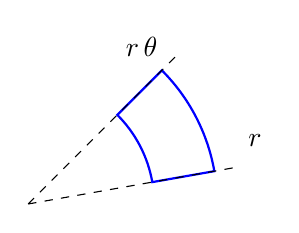
\begin{tikzpicture}[scale=.8]
\draw[blue,thick] (10:2) arc(10:45:2)--(45:3) arc(45:10:3)--cycle;
\draw[dashed] (0,0)--(45:3.3) (0,0)--(10:3.3);
\node at (3.6,1) {$\dd r$}; \node at (1.8,2.5) {$r\,\dd\theta$};
\end{tikzpicture}
\end{center}

\begin{example}[Polar coordinates and the unit disk]
Consider
\[
\sigma(\theta,r)=(r\cos\theta,r\sin\theta).
\]
Its derivative is represented by the Jacobian
\[
J_\sigma(\theta,r)=
\begin{pmatrix}
-r\sin\theta&\cos\theta\\
r\cos\theta&\sin\theta
\end{pmatrix},
\qquad
\det D\sigma(\theta,r)=-r,\qquad\abs{\det D\sigma(\theta,r)}=r.
\]
The parameter order $(\theta,r)$ specifies the two Jacobian columns.
Compared with the order $(r,\theta)$ in \cref{ex:polar-jacobian}, this
swaps columns: the determinant changes from $+r$ to $-r$, while its
absolute value remains $r$.
The nested notation $\dd r\,\dd\theta$ instead instructs us to integrate
in $r$ first, then $\theta$. Exchanging legitimate scalar iterated integrals
has no minus sign; exchanging wedge factors does. The order $(\theta,r)$
reverses orientation, while the absolute determinant for scalar area remains positive.
The geometric preview above used actual increments: an angular
change $\Delta\theta$ at radius $r$ sweeps an arc of length approximately
$r\Delta\theta$, while a radial change has length $\Delta r$.
The present theorem supplies the rigorous integral statement.

To use the theorem without hiding its hypotheses, first take
\[
Q_{\varepsilon,\eta}=[\eta,2\pi-\eta]\times[\varepsilon,1]
\]
with $\varepsilon,\eta>0$.  On this rectangle the map is injective and its
Jacobian determinant never vanishes.  Its image is an annular sector.  For example,
since $x^2+y^2=r^2$,
\begin{align*}
\int_{\sigma(Q_{\varepsilon,\eta})}(x^2+y^2)\,\dd(x,y)
&=\int_\eta^{2\pi-\eta}\int_\varepsilon^1r^2\,r\,\dd r\,\dd\theta\\
&=\frac{(2\pi-2\eta)(1-\varepsilon^4)}4.
\end{align*}
Letting $\varepsilon,\eta\to0^+$ gives
\[
\int_{x^2+y^2\leq1}(x^2+y^2)\,\dd(x,y)=\frac\pi2.
\]
The following discarded-area bounds are deliberately independent of the
disk area already computed by Cartesian slices. The central disk lies in $[-\varepsilon,\varepsilon]^2$,
so its area is at most $4\varepsilon^2$. For $0<\eta<\pi/2$, the omitted
angular seam has $0\leq x\leq1$ and $|y|\leq\sin\eta\leq\eta$;
it lies in $[0,1]\times[-\eta,\eta]$, of area $2\eta$.
Their combined outer area is at most $4\varepsilon^2+2\eta\to0$.
The integrand is bounded by $1$, so the discarded integrals obey the same
bound. The unit circle is Jordan-null independently, by the Lipschitz
image-of-an-interval estimate applied to $(\cos t,\sin t)$ on $[0,2\pi]$;
thus the disk's Jordan measurability also precedes its area calculation.  The
same calculation with integrand $1$ recovers the disk-area formula by a
second method:
\[
\int_{x^2+y^2\leq1}1\,\dd(x,y)=\pi.
\]
\end{example}




% Original vector figure for Version 3.9.0.
\begin{figure}[htbp]
\centering
\begin{tikzpicture}[font=\small,>=Stealth,line width=.65pt]
\filldraw[fill=blue!8,draw=blue] (0,0) rectangle(1.2,1);
\fill (0,0) circle(1.5pt) node[below] {$a$};
\node[above] at (.6,1) {small source cell};
\draw[->] (1.6,.5)--(2.8,.5) node[midway,above] {$\sigma$};
\begin{scope}[xshift=3.3cm]
\filldraw[fill=blue!8,draw=blue,thick] (0,0)--(1.5,.25) .. controls (1.9,.6) and (2,1.1) .. (1.9,1.4) .. controls (1.3,1.35) and (.7,1.2) .. (.35,1.05) .. controls (.2,.7) and (.1,.3) .. (0,0);
\draw[orange!85!black,dashed,thick] (0,0)--(1.5,.25)--(1.85,1.3)--(.35,1.05)--cycle;
\fill (0,0) circle(1.5pt) node[below] {$\sigma(a)$};
\node[below,align=center] at (1,-.6) {dashed: $\sigma(a)+D\sigma(a)h$};
\node[right,blue] at (2,1.4) {nonlinear image};
\end{scope}
\end{tikzpicture}
\caption{The derivative gives a first-order parallelogram model, not an exact image. Its area is $|\det D\sigma(a)|$ times the source area; the nonlinear error is controlled as the cell shrinks.}\label{fig:jacobian-distortion}
\end{figure}

\subsection{Worked changes of variables}
\begin{center}
\fbox{\parbox{.88\linewidth}{\textbf{Computational checklist.}
Choose coordinates and write the source-to-target map $\sigma$; describe the
source domain; compute $D\sigma$ and $|\det D\sigma|$; substitute in the
integrand; check the hypotheses or controlled exceptions; evaluate.}}
\end{center}
Classical analytic geometry asks which coordinates make a curve, surface,
or region's equation simplest. Change of variables asks the same question
simultaneously for the domain and the integrand. A disk suggests polar
coordinates, an ellipse suggests scaling, the linear expressions $x+y,x-y$
suggest oblique coordinates, and a cone suggests cylindrical coordinates.

\begin{example}[Two substitutions for an ellipse]
Use \cref{ex:ellipse-scaling}. For $f(x,y)=x^2/a^2+y^2/b^2$,
$f(\sigma(u,v))=u^2+v^2$ and $|\det D\sigma|=ab$. On the source disk
use $(u,v)=(r\cos\theta,r\sin\theta)$, now with parameter order
$(r,\theta)$ and determinant $r$. The preceding polar truncation justifies
the seam and central-point exceptions. Thus
\[
\int_E f\,\dd(x,y)=ab\int_0^{2\pi}\int_0^1 r^2r\,\dd r\,\dd\theta
=\frac{\pi ab}{2}.
\]
The two absolute Jacobian determinant factors describe two successive changes of coordinates.
\end{example}
\begin{example}[Linear expressions as coordinates]
On $E=\{|x+y|\leq1,\ |x-y|\leq1\}$ put $u=x+y$, $v=x-y$.
Solving for the old variables gives the required source-to-target map
\[
\sigma(u,v)=((u+v)/2,(u-v)/2),\quad (u,v)\in[-1,1]^2,
\qquad D\sigma=\tfrac12\begin{pmatrix}1&1\\1&-1\end{pmatrix}.
\]
It is globally invertible and $|\det D\sigma|=1/2$, whereas the inverse
coordinate map has absolute determinant $2$. For the adapted integrand,
\[
\int_E\bigl((x+y)^2+(x-y)^2\bigr)\,\dd(x,y)
=\frac12\int_{-1}^1\int_{-1}^1(u^2+v^2)\,\dd v\,\dd u=\frac43.
\]
\noindent\begin{minipage}{\linewidth}
\begin{center}
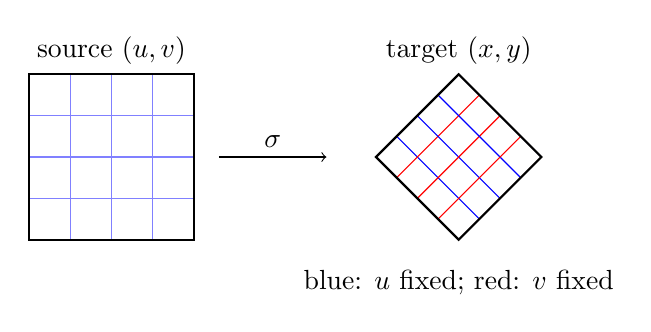
\begin{tikzpicture}[scale=1.05]
\draw[step=.5,blue!50] (-1,-1) grid(1,1);
\draw[thick] (-1,-1) rectangle(1,1);
\node[above] at (0,1) {source $(u,v)$};
\draw[->] (1.3,0)--(2.6,0) node[midway,above] {$\sigma$};
\begin{scope}[xshift=4.2cm]
\foreach \t in {-1,-.5,0,.5,1}{
\draw[blue] ({(\t-1)/2},{(\t+1)/2})--({(\t+1)/2},{(\t-1)/2});
\draw[red] ({(-1+\t)/2},{(-1-\t)/2})--({(1+\t)/2},{(1-\t)/2});}
\draw[thick] (-1,0)--(0,1)--(1,0)--(0,-1)--cycle;
\node[above] at (0,1) {target $(x,y)$};
\node[below] at (0,-1.25) {blue: $u$ fixed; red: $v$ fixed};
\end{scope}
\end{tikzpicture}
\end{center}
Good coordinates simplify both the domain and the integrand: the oblique
lines become coordinate lines on the source square.
\end{minipage}
\end{example}
\begin{example}[A rectangle becomes a trapezoid]
Take $\sigma(u,v)=(u,(1+u)v)$ on $Q=[0,1]^2$. Its image is
$E=\{0\leq x\leq1,\ 0\leq y\leq1+x\}$, and
\[
D\sigma=\begin{pmatrix}1&0\\v&1+u\end{pmatrix},\qquad \det D\sigma=1+u.
\]
The inverse is $(x,y)\mapsto(x,y/(1+x))$, smooth on $x>-1$.
For $f(x,y)=y$, there are two separate transformations:
\[
f(\sigma(u,v))=(1+u)v,\qquad \dd(x,y)=(1+u)\,\dd(u,v).
\]
Therefore
\[
\int_E y\,\dd(x,y)=\int_0^1\int_0^1(1+u)^2v\,\dd v\,\dd u
=\frac12\int_0^1(1+u)^2\,\dd u=\frac76.
\]
With integrand $1$ the area is $\int_0^1(1+u)\,\dd u=3/2$.
\begin{center}
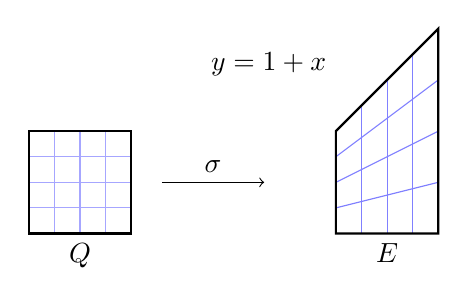
\begin{tikzpicture}[scale=1.3]
\draw[step=.25,blue!35] (0,0) grid (1,1);\draw[thick] (0,0) rectangle(1,1);
\node[below] at (.5,0) {$Q$};
\draw[->] (1.3,.5)--(2.3,.5) node[midway,above] {$\sigma$};
\begin{scope}[xshift=3cm]
\foreach \u in {0,.25,.5,.75,1}{\draw[blue!50] (\u,0)--(\u,{1+\u});}
\foreach \v in {0,.25,.5,.75,1}{\draw[blue!50] (0,\v)--(1,{2*\v});}
\draw[thick] (0,0)--(1,0)--(1,2)--(0,1)--cycle;
\node[left] at (0,1.65) {$y=1+x$};\node[below] at (.5,0) {$E$};
\end{scope}
\end{tikzpicture}
\end{center}
Horizontal coordinate lines $v=\text{constant}$ become sloping lines.
\end{example}
\begin{example}[A radial integrand]
For $R>0$, polar coordinates transform $x^2+y^2\leq R^2$ into
$0\leq r\leq R$, $0\leq\theta\leq2\pi$, subject to the same controlled
seam and center exceptions as before. Since $(x^2+y^2)^2=r^4$,
\[
\int_{x^2+y^2\leq R^2}(x^2+y^2)^2\,\dd(x,y)
=\int_0^{2\pi}\int_0^R r^5\,\dd r\,\dd\theta=\frac{\pi R^6}{3}.
\]
\begin{center}
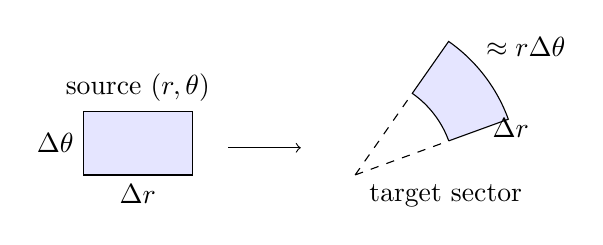
\begin{tikzpicture}[scale=1.15]
\draw[fill=blue!10] (0,0) rectangle(1.2,.7);
\node[below] at (.6,0) {$\Delta r$};\node[left] at (0,.35) {$\Delta\theta$};
\node[above] at (.6,.7) {source $(r,\theta)$};
\draw[->] (1.6,.3)--(2.4,.3);
\begin{scope}[xshift=3cm]
\filldraw[fill=blue!10] (20:1.1)--(20:1.8) arc(20:55:1.8)--(55:1.1) arc(55:20:1.1);
\draw[dashed] (0,0)--(20:1.1) (0,0)--(55:1.1);
\node[right] at (20:1.5) {$\Delta r$};
\node[above right] at (42:1.8) {$\approx r\Delta\theta$};
\node[below] at (1,0) {target sector};
\end{scope}
\end{tikzpicture}
\end{center}
The two small side lengths explain the area factor $r$; the theorem
turns this first-order picture into an exact integral formula.
\end{example}
\begin{example}[Cylindrical coordinates revisit the cone]
Use $\sigma(r,\theta,z)=(r\cos\theta,r\sin\theta,z)$. With this parameter order,
\[
D\sigma=\begin{pmatrix}\cos\theta&-r\sin\theta&0\\
\sin\theta&r\cos\theta&0\\0&0&1\end{pmatrix},\qquad \det D\sigma=r.
\]
The cone in \cref{ex:cylinder-cone-slices} has source bounds
$0\leq z\leq h$, $0\leq\theta\leq2\pi$, $0\leq r\leq R(1-z/h)$.
On $r>0$, $0<\theta<2\pi$ the map is a diffeomorphism onto the slit
space. For $0<\varepsilon<R$ and $0<\eta<\pi/2$, retain the compact source
\[
\begin{split}
E_{\varepsilon,\eta}=\{(r,\theta,z):\ &0\leq z\leq h(1-\varepsilon/R),\quad
\eta\leq\theta\leq2\pi-\eta,\\
&\varepsilon\leq r\leq R(1-z/h)\}.
\end{split}
\]
The shortened height range follows by solving
$\varepsilon\leq R(1-z/h)$ for $z$; it prevents reversed radial bounds near
the apex. This Jordan region lies inside the diffeomorphism domain, so
\cref{cor:jordan-nonlinear-change} applies. The omitted target lies in a
central box of volume $4\varepsilon^2h$ and a seam box of volume at most
$2R^2\eta h$. Their volumes tend to zero. The nonnegative omitted source
integral, including the small apex portion, is at most
\[
\int_0^h\int_0^{2\pi}\int_0^\varepsilon r\,\dd r\,\dd\theta\,\dd z
+2\eta\int_0^h\int_0^R r\,\dd r\,\dd z
=\pi h\varepsilon^2+\eta hR^2\longrightarrow0.
\]
Hence
\[
\operatorname{vol}(K)=\int_0^h\int_0^{2\pi}
\int_0^{R(1-z/h)}r\,\dd r\,\dd\theta\,\dd z
=\pi R^2\int_0^h(1-z/h)^2\,\dd z=\frac13\pi R^2h.
\]
The inner two integrals recover the disk area at height $z$. This is the
same solid and the same answer as cross-sectional Fubini. Geometrically,
a small cylindrical cell has side lengths $\Delta r$, approximately
$r\Delta\theta$, and $\Delta z$, explaining its volume factor $r$.
\end{example}
\begin{example}[Spherical coordinates and the ball]\label{ex:spherical-ball}
Use the parameter order $(\rho,\varphi,\theta)$ and the convention
\[
\sigma(\rho,\varphi,\theta)=
(\rho\sin\varphi\cos\theta,\rho\sin\varphi\sin\theta,\rho\cos\varphi).
\]
Here $\rho\geq0$ is distance from the origin, $0\leq\varphi\leq\pi$
is the angle from the positive $z$-axis, and $0\leq\theta<2\pi$ is
the azimuthal angle in the $xy$-plane. Differentiating in this order gives
\[
D\sigma=\begin{pmatrix}
\sin\varphi\cos\theta&\rho\cos\varphi\cos\theta&-\rho\sin\varphi\sin\theta\\
\sin\varphi\sin\theta&\rho\cos\varphi\sin\theta&\rho\sin\varphi\cos\theta\\
\cos\varphi&-\rho\sin\varphi&0
\end{pmatrix}.
\]
Expansion of the determinant gives $\det D\sigma=\rho^2\sin\varphi$,
which is nonnegative on the stated parameter ranges.
For $R>0$ the resulting formula is
\[
\operatorname{vol}(B_R)=\int_0^R\int_0^\pi\int_0^{2\pi}
\rho^2\sin\varphi\,\dd\theta\,\dd\varphi\,\dd\rho
=\frac43\pi R^3.
\]
Here is the justification at the coordinate exceptions. The map is a
diffeomorphism on $\rho>0$, $0<\varphi<\pi$, $0<\theta<2\pi$ onto
the complement of the polar axis and angular seam: recover $\rho$ as
the norm, $\varphi=\arccos(z/\rho)$, and the unique azimuth in that interval.
These inverses are smooth locally. At the origin all angles coincide;
on the polar axis azimuth is undetermined; and the closed angular box
repeats the seam at $\theta=0,2\pi$. Thus the full box is not a global
diffeomorphism domain.

Apply \cref{cor:jordan-nonlinear-change} first on
$[\delta,R]\times[\eta,\pi-\eta]\times[\eta,2\pi-\eta]$,
where $0<\delta<R$ and $0<\eta<\pi/2$. The omitted target lies in
a central cube of volume $8\delta^3$, an axis box of volume at most
$8R^3\sin^2\eta$, and a seam slab of volume at most $4R^3\sin\eta$.
These tend to zero. The omitted nonnegative source integral is bounded by
\[
\frac{4\pi}{3}\delta^3+
\frac{4\pi R^3}{3}(1-\cos\eta)+\frac{4\eta R^3}{3},
\]
which also tends to zero. The sphere bounding the ball is Jordan-null:
it is the Lipschitz image under $\sigma(R,\cdot,\cdot)$ of a parameter
rectangle, by the earlier lower-dimensional image theorem. Hence the
ball is Jordan measurable and its open and closed versions have equal
volume. This completes the same truncation argument used for polar and
cylindrical coordinates, without discarding a coordinate exception silently.
\end{example}
% Original vector figure for Version 3.9.0.
\begin{figure}[htbp]
\centering
\begin{tikzpicture}[font=\small,>=Stealth,line width=.65pt]
\begin{scope}[x={(1cm,-.2cm)},y={(.5cm,.45cm)},z={(0cm,1cm)}]
\draw[->,gray] (0,0,0)--(2.8,0,0) node[right] {$x$};
\draw[->,gray] (0,0,0)--(0,2.6,0) node[right] {$y$};
\draw[->,gray] (0,0,0)--(0,0,2.6) node[above] {$z$};
\coordinate (P) at (1.5,1.3,1.8);
\draw[->,blue,thick] (0,0,0)--(P) node[pos=.75,left] {$\rho$};
\draw[dashed] (P)--(1.5,1.3,0)--(0,0,0);
\draw[red!80!black] plot[domain=0:40.9,samples=24] ({.85*cos(\x)},{.85*sin(\x)},0);
\node at (.95,.3,0) [below] {$\theta$};
\draw[orange!80!black] plot[domain=0:47.8,samples=24] ({.8*sin(\x)*.7557},{.8*sin(\x)*.6549},{.8*cos(\x)});
\node at (.25,.2,.95) [right] {$\varphi$};
\fill (P) circle(2pt) node[right] {$\sigma(\rho,\varphi,\theta)$};
\end{scope}
\node[align=left] at (5.9,1.6) {$\varphi$: from $+z$\\$\theta$: azimuth from $+x$};
\end{tikzpicture}
\caption{Our spherical-coordinate convention. The dashed vertical segment projects the point to the $xy$-plane. The polar angle is measured from the positive $z$-axis.}\label{fig:spherical-coordinates}
\end{figure}

\begin{center}
\fbox{\parbox{.88\linewidth}{\textbf{Change-of-variables warnings.}
Transform the integrand \emph{and} the domain and include the absolute Jacobian determinant.
Do not retain old bounds after substitution, or omit the absolute Jacobian determinant after
changing bounds. For $\sigma$ from new coordinates to old, the factor is
$|\det D\sigma|$, not the determinant of the inverse map. Ordinary scalar
area and volume use an absolute value. Verify injectivity and control
singular-coordinate exceptions. Oriented forms instead keep a sign.}}
\end{center}

\section{Convergence and Multiple Integration}

The same principle from Chapter~9 survives unchanged on a rectangle: a
uniform error in the integrand is at most that error times the volume of the
domain after integration.  Pointwise convergence alone is not the Riemann
theory's general interchange principle.

\begin{theorem}[Uniform interchange for multiple Riemann integrals]
\label{thm:uniform-multivariable-riemann}
Let \(Q\subseteq\R^n\) be a rectangle.  Suppose that every function
\[
f_k:Q\longrightarrow\R
\]
is Riemann integrable and that \(f_k\) converges uniformly to \(f\) on
\(Q\).  Then \(f\) is Riemann integrable and
\[
\lim_{k\to\infty}\int_Qf_k(x)\,\dd x
=
\int_Qf(x)\,\dd x.
\]
Moreover,
\[
\lim_{k\to\infty}\int_Q\abs{f_k(x)-f(x)}\,\dd x=0.
\]
\end{theorem}
\begin{proof}
The oscillation argument in the proof of
\cref{thm:uniform-riemann-integration} applies to grid subrectangles, using
\cref{prop:multivariable-darboux}. Explicitly the bound is
$U(f,\mathcal P)-L(f,\mathcal P)\leq
U(f_k,\mathcal P)-L(f_k,\mathcal P)+2\|f-f_k\|_\infty\operatorname{vol}(Q)$:
the interval length in Chapter~9 has become volume.  Once integrability of \(f\) is known,
\cref{thm:multivariable-integral-properties} gives
\[
\left\lvert\int_Qf_k\,\dd x-\int_Qf\,\dd x\right\rvert
\leq
\int_Q\abs{f_k-f}\,\dd x
\leq
\operatorname{vol}(Q)\sup_{x\in Q}\abs{f_k(x)-f(x)}.
\]
The right-hand side tends to zero, and the same estimate gives the final
claim.
\end{proof}

The uniform theorem gives
\[
\int_Q|f_k-f|\leq\operatorname{vol}(Q)\|f_k-f\|_\infty\longrightarrow0.
\]
Thus uniform convergence gives $L^1$ convergence (convergence of the
integral of the absolute error), then convergence of integrals. The same
result holds on a Jordan region for integrable functions: extend all maps
by zero to one containing rectangle. Their uniform errors remain bounded
by the original error, so the rectangular theorem applies.

\subsection{Arzel\`a bounded convergence on rectangles}
The proof of \cref{thm:arzela-bounded-riemann} used open interval lengths
and compact inner approximations. Its replacement dictionary is
\begin{center}
\begin{tabular}{p{0.43\linewidth}p{0.43\linewidth}}
\textbf{Chapter 9: intervals}&\textbf{Here: rectangles}\\
Open-set length $\ell(G)$&Open-box content $c(G)$\\
Finite unions of closed intervals&Finite unions of closed boxes\\
Nested open sets of uniformly positive length&Nested open sets of uniformly positive content
\end{tabular}
\end{center}
The following lemma proves the new box geometry. Once it is available,
the bounded-height, large-error-region contradiction is the same one.
For open $G\subset Q^\circ$, let $c(G)$ be the supremum of the total
volumes of finite families of closed boxes contained in $G$ with pairwise
disjoint interiors; include the empty family, of volume zero.
Every such total is at most $\operatorname{vol}(Q)$, by a common grid.
\begin{lemma}[Open-box content tools]\label{lem:open-box-content}
For open subsets of $Q^\circ$, the following hold:
\begin{enumerate}[label=(\arabic*)]
\item If $G\subseteq\bigcup_jG_j$, then $c(G)\leq\sum_jc(G_j)$.
\item Given $\eta>0$, there is a finite union $K$ of closed boxes in $G$
with $c(G\setminus K)<\eta$.
\item If open $G_N$ decrease and $c(G_N)\geq c_0>0$ for every $N$,
then $\bigcap_N G_N$ is nonempty.
\end{enumerate}
\end{lemma}
\begin{proof}
Compare only finite box families, and use compactness to
turn open covers into finite subdivisions.
For (1), take any admissible compact box union $K\subset G$. A finite
subcover from the $G_j$ covers $K$. A Lebesgue number for this compact
cover (\cref{lem:compact-metric-lebesgue-number}) permits subdivision of its boxes into closed cells, each contained
in one chosen $G_j$. The common-scale argument is proved in
\cref{lem:sequential-cover-mechanisms}. Assign each cell to one such $j$.
The cells assigned to a given $j$ have disjoint interiors and lie in $G_j$,
so their total is at most $c(G_j)$. Sum and take the supremum over $K$.
For (2), choose an admissible $K$ of volume greater than $c(G)-\eta$.
Any admissible box family in $G\setminus K$ can be joined to the boxes
of $K$ and still lies in $G$ with disjoint interiors. Its total is at
most $c(G)-\operatorname{vol}(K)<\eta$; the same bound holds for its
supremum. Here volume of a finite box union means its finite grid volume.

For (3), choose $K_i\subset G_i$ as in (2) with error $c_0/2^{i+1}$.
The compact sets $H_N=K_1\cap\cdots\cap K_N$ decrease. If $H_N$ were
empty, nesting would imply
$G_N\subseteq\bigcup_{i=1}^N(G_i\setminus K_i)$; (1) would give
$c(G_N)<c_0/2$, a contradiction. Thus all $H_N$ are nonempty and
compact; their intersection is nonempty by compactness, and lies in every $G_N$.
\end{proof}
For a finite collection of boxes with disjoint interiors, the content of
the union of their interiors equals the sum of their volumes: shrink each
box slightly for the lower bound, and subdivide a finite test family with
the box faces for the upper bound. This identifies the numerical content
needed in the next proof; it does not assert Jordan measurability of arbitrary open sets.

\begin{theorem}[Multivariable Arzel\`a bounded convergence]\label{thm:multivariable-arzela-bounded}
Let $Q$ be a compact rectangle, let $f_k:Q\to\R$ be Riemann integrable,
and suppose $f_k\to f$ pointwise and $|f_k(x)|\leq M$ for all $k,x$.
Assume separately that $f$ is Riemann integrable. Then
\[
\int_Q|f_k-f|\longrightarrow0,\qquad \int_Q f_k\longrightarrow\int_Q f.
\]
\end{theorem}
\begin{proof}
A large integral with bounded heights forces large open
error regions; compact inner approximations force one point into arbitrarily
late regions, contradicting pointwise convergence.
Set $g_k=|f_k-f|$. The integral algebra makes $g_k$ integrable and
$0\leq g_k\leq2M$, since the pointwise limit also satisfies $|f|\leq M$.
The case $M=0$ is immediate. Otherwise replace $g_k$ by $g_k/(2M)$,
so $0\leq g_k\leq1$. Write $V=\operatorname{vol}(Q)>0$.
If its integrals do not tend to zero, select a subsequence with
$\int_Qg_k>2\eps V$ for one fixed $\eps>0$.
Choose a lower sum exceeding $2\eps V$. Cells of lower height at most
$\eps$ contribute at most $\eps V$; the remaining cells therefore
have combined volume greater than $\eps V$, since their heights are at most one.
Let $U_k$ be the union of their interiors. Then $c(U_k)>\eps V$ and
$g_k(x)>\eps$ throughout $U_k$. The open sets
$G_N=\bigcup_{k\geq N}U_k$ decrease and each has content at least $\eps V$.
By \cref{lem:open-box-content}, there is a fixed $x\in\bigcap_NG_N$.
For every $N$ some $k\geq N$ then satisfies $g_k(x)>\eps$, contrary to
$g_k(x)\to0$. Undoing the height normalization proves the first limit.
Finally $|\int_Q f_k-\int_Q f|\leq\int_Q|f_k-f|$ proves the second.
\end{proof}
Uniform convergence controls the whole domain by one error bound.
Arzel\`a bounded convergence uses compactness to prevent regions of large
error and substantial content from moving forever without revisiting a
fixed point. The integrability of the limit is still a separate assumption.
For example $f_k(x,y)=x^k$ on $[0,1]^2$ has a limit supported on the face
$x=1$, hence integrable with integral zero by the face-strip lemma.
The convergence is not uniform, but this theorem gives integral convergence;
direct calculation yields $\int f_k=1/(k+1)$.



As in one variable, pointwise convergence alone does not control a Riemann
integral.  On a compact rectangle, continuity and monotonicity provide the
extra structure that can force uniform convergence.
The proof of \cref{thm:dini-riemann} applies: continuity makes the good
sets relatively open, monotonicity makes them nested, and compactness
reduces their cover to one uniform index. No ordering of the domain is used.

\begin{theorem}[Dini's theorem]
\label{thm:dini-multivariable-riemann}
Let \(Q\subseteq\R^n\) be a rectangle, and let
\[
f_k:Q\longrightarrow\R
\]
be continuous functions satisfying
\[
f_k(x)\leq f_{k+1}(x)
\qquad(x\in Q,\ k\in\N).
\]
If \(f_k\) converges pointwise on \(Q\) to a continuous function \(f\),
then the convergence is uniform and
\[
\lim_{k\to\infty}\int_Qf_k(x)\,\dd x
=
\int_Qf(x)\,\dd x.
\]
The same conclusion holds for a pointwise decreasing sequence.
\end{theorem}
\begin{proof}
\textbf{Strategy.} Nested open good sets turn a finite subcover into one
uniform index. In the increasing case set $h_n=f-f_n\geq0$ on $K=Q$.
For $\eps>0$, the relatively open sets
\[
U_n=\{x\in K:h_n(x)<\eps/2\}
\]
are increasing, and pointwise convergence gives $K=\bigcup_n U_n$.
Compactness of $K$ supplies a finite subcover. Its largest-index member
$U_N$ already covers $K$. For $n\geq N$ and every $x\in K$,
$0\leq h_n(x)<\eps/2$, hence $\sup_K|f-f_n|\leq\eps/2<\eps$.
This proves uniform convergence, and \cref{thm:uniform-multivariable-riemann} gives the integral formula.
Apply the increasing case to $-f_n$ for a decreasing sequence.
\end{proof}

\begin{remark}[Which convergence theorem applies?]
Uniform interchange assumes integrable approximants and uniform convergence;
it proves integrability of the limit and bounds the absolute-error integral
by volume times the uniform error. Arzel\`a assumes pointwise convergence,
a common bound, and separately an integrable limit; compact inner box
approximations give convergence of absolute-error integrals.
Dini assumes continuous approximants, a continuous limit, monotonicity,
and compactness; these first give uniform convergence, then integral convergence.
The later Lebesgue dominated convergence theorem instead uses measurable
functions, almost-everywhere convergence, and an integrable dominating
function; in that different theory it also supplies integrability of the limit.
It is not the uniform theorem under another name and is not proved here.
\end{remark}

\section*{Exercises}
\begin{exercise}
For $P(x,t)=(x,e^xt)$ and $f\in C_c(\R^2)$, prove the substitution
formula directly by integrating in $t$ first. Explain the support of
the pulled-back integrand and the factor $e^x$.
\end{exercise}

\addcontentsline{toc}{section}{Exercises}

\begin{exercise}
Prove that replacing a grid partition by a refinement decreases its upper
sum and increases its lower sum.
\end{exercise}

\begin{exercise}
Compute
\[
\int_{\{0\leq y\leq1,\ y\leq x\leq y+2\}}(x+2y)\,\dd(x,y)
\]
directly from iterated one-variable integrals.
\end{exercise}

\begin{exercise}
Use \cref{thm:coordinatewise-integration-by-parts} with \(j=1\) to
evaluate
\[
\int_{[0,1]^2}x\frac{\partial}{\partial x}(x^2y)\,\dd(x,y).
\]
\end{exercise}

\begin{exercise}
Prove that a constant function $c$ on $Q$ has integral
\[
c\operatorname{vol}(Q).
\]
\end{exercise}

\begin{exercise}
Show that a finite set in $\R^n$ has Jordan volume zero.
\end{exercise}

\begin{exercise}
Prove that the open unit ball in $\R^n$ is Jordan measurable, assuming that
its boundary can be covered by finitely many boxes of arbitrarily small total
volume.
\end{exercise}

\begin{exercise}
Give a bounded subset of $[0,1]$ whose indicator is not Riemann integrable.
\end{exercise}

\begin{exercise}
Use \cref{thm:linear-change-variables} to compute the area of the
parallelogram spanned by two vectors in $\R^2$.
\end{exercise}

\begin{exercise}
Verify the determinant computation in the polar-coordinate example.
\end{exercise}

\begin{exercise}
For $a,b>0$, use a linear map and polar coordinates to compute
\[
\int_{\{x^2/a^2+y^2/b^2\leq1\}}
x^2\,\dd(x,y).
\]
Transform the domain and both scaling factors. Justify the exceptional
origin and angular seam by truncation and bounds, as in the disk example.
\end{exercise}


\section{Strategy for Multiple Integrals: Geometry, Coordinates, and Computation}
Existence and evaluation are different tasks. The chapter's continuity,
Darboux, and Jordan results establish existence; the following procedure
helps choose an efficient evaluation using those results.
\begin{enumerate}[label=\arabic*.]
\item \textbf{Identify dimension and meaning.} Is this a double integral
over $E\subset\R^2$ or a triple integral over $\Omega\subset\R^3$?
Integrand $1$ computes area or volume; a density computes total mass.
\item \textbf{Draw and label the set.} Mark boundaries, intersection
points, axes, symmetries, and a representative slice. For a solid, include
the projection region that will carry the outer integral.
\item \textbf{Try slicing.} Compare vertical and horizontal slices in
the plane. In space compare horizontal cross-sections with projections
onto the $xy$, $xz$, and $yz$ planes. Solve the inequalities for the inner
variable; the picture helps detect missing bounds.
\item \textbf{Split where a boundary changes.} The roof-shaped triangle
requires two vertical descriptions but only one horizontal description.
Two simple integrals can be clearer than one complicated bound.
\item \textbf{Use symmetry precisely.} Name a transformation preserving
the domain and check how the integrand changes. For example if
$(x,y)\mapsto(-x,y)$ preserves $E$ and $f(-x,y)=-f(x,y)$, its absolute
Jacobian determinant is $1$ and substitution gives $\int_Ef=-\int_Ef=0$.
\item \textbf{Look for adapted coordinates.} Expressions $x^2+y^2$
suggest polar or cylindrical coordinates; ellipses suggest scaling;
$x+y$ and $x-y$ boundaries suggest using those expressions as coordinates.
The best substitution simplifies the domain, the integrand, or ideally both.
\item \textbf{Check the substitution.} Write $\sigma$,
the parameter domain, $D\sigma$, $|\det D\sigma|$, the transformed integrand,
and the hypotheses or controlled exceptions before integrating.
\item \textbf{Check the answer.} Area and volume are nonnegative and no
larger than those of containing boxes. If $0\leq f\leq M$, then
$0\leq\int_Ef\leq M\operatorname{vol}(E)$. Scaling every length by
$c>0$ scales $n$-dimensional volume by $c^n$.
\end{enumerate}
For the cone, cross-sections immediately give $A(z)=\pi R^2(1-z/h)^2$.
Cylindrical coordinates instead compute that area as the inner two
integrals and accommodate densities depending on $r,\theta,z$ naturally.
Neither method is universally superior. Choose the description in which
the geometry and the resulting integral are easiest to handle.

\begin{exercise}[Choose and justify a method]
\begin{enumerate}
\item Reverse the order in the picture of \cref{ex:parabolic-slices} and
compute $\int_E x^2$. Label a representative slice of each kind.
\item Compute the volume of $0\leq z\leq h$, $x^2+y^2\leq R^2z/h$
by cross-sections, and independently by cylindrical coordinates.
\item Find the volume of $x^2/4+y^2/9+z^2/16\leq1$ by scaling.
\item On $|x+y|\leq2$, $|x-y|\leq1$, integrate $(x+y)^2$ using these
two linear expressions as coordinates.
\item Compare Cartesian, polar, and symmetry methods for
$\int_{x^2+y^2\leq1}x$ and for $\int_{x^2+y^2\leq1}(x^2+y^2)$.
Explain which steps each choice saves.
\end{enumerate}
\end{exercise}

\section{Limits of the Riemann Theory}

The Riemann integral handles continuous functions and geometrically regular
domains very effectively.  Its limitations become sharper in several
variables: indicators of sets with complicated boundaries may fail to be
integrable, iterated integrals need not be available for arbitrary bounded
functions, and the present change-of-variables theorem requires continuity
and a globally injective parametrization.  Lebesgue measure and integration
replace Jordan volume by a much more flexible notion of size and later permit
theorems under substantially weaker hypotheses.  Those extensions are not
developed in these notes.
